%%%%%%%%%%%%%%%%%%%%%%%%%%%%%%%%%%%%%%%%%%%%%%%%%%%%%%%%%%%%%%%%%%%%%%%%%%%%%%%
%%%%%%%%%%%%%%%%%%%%%%%%%%%%%%%%%%%%%%%%%%%%%%%%%%%%%%%%%%%%%%%%%%%%%%%%%%%%%%%
%%%%  CHAPTER 4   
%%%%%%%%%%%%%%%%%%%%%%%%%%%%%%%%%%%%%%%%%%%%%%%%%%%%%%%%%%%%%%%%%%%%%%%%%%%%%%%
%%%%%%%%%%%%%%%%%%%%%%%%%%%%%%%%%%%%%%%%%%%%%%%%%%%%%%%%%%%%%%%%%%%%%%%%%%%%%%%
\chapter{Overview of the experimental setup}
\label{chap:setup-overview}

In this chapter we will give a brief description of the experimental setup used
for this thesis.  The idea is to make the reader familiar with the experimental
steps required to produce an ultracold Fermi gas and the different systems
associated with each step,  before explaining concepts in more detail in later
chapters.  We will assume familiarity with the use of light to cool and trap
atoms~\cite{RevModPhys.70.685,RevModPhys.70.707,RevModPhys.70.721},  and with
the use of magnetic fields to control the strength of the interactions between
atoms~\cite{RevModPhys.82.1225}. 

For the non-expert, it will suffice to know that light that is near resonant to
an atomic transition can result in dissipative forces, which can be used to
reduce the velocity of atoms (cooling).  Light detuned far from an atomic
transition produces a conservative force,  which changes the potential energy
of an atom.  If the far detuned light is detuned to the red of the atomic
transition, atoms will be attracted to intensity maxima of the light field
(trapping), whereas if the light is red detuned they will be repelled from the
intensity maxima. 


It takes about 15 seconds to produce a degenerate cloud of \li\ atoms.  It then
takes only a few tens of milliseconds to load this cold sample into an optical
lattice and perform a measurement on it.  Measurements are destructive, so we
must repeat the process over and over again.   Most of the time in the lab is
spent optimizing the setup and finding out the right way to carry out the
experiments.   Final data can then consist of only a few tens to a few hundred
shots, depending on the statistics needed for the particular experiment. 

In Fig.~\ref{fig:vacuum} we show a schematic of the vacuum system where the
experiments are carried out.  This will give the reader a spatial setting in
which to visualize the descriptions given below.  The experimental cycle
proceeds in the following way:  
\begin{enumerate} 
\item A thermal beam of \li\ atoms, which originates at the oven, is
decelerated by near-resonant counter-propagating light.  A tapered solenoid is
used to produce a spatially varying magnetic field used to compensate the
changing Doppler shift as the atoms decelerate.   This scheme is referred to as
Zeeman slowing.  After the Zeeman slower, the atoms are  cooled transversally
by the two-dimensional magneto-optical trap (2DMOT). 

\item  The magneto-optical trap (MOT) captures the slowed atoms at the center
of the chamber, where they reach a temperature as low as $\sim300~\mu$K.  

\item  We transfer the atoms from the MOT to a narrow linewidth magneto-optical
trap, which operates on the ultraviolet \uv\ transition (UVMOT).  In the UVMOT
the atoms are cooled down to $\sim60~\mu$K.  

\item  We load a balanced mixture of atoms in the two lowest energy hyperfine
states into a crossed-beam optical dipole trap (ODT)

\item  Once in the ODT, a magnetic field is used to control the scattering
cross section between atoms in the two different hyperfine states, via a
magnetic Feshbach resonance~\cite{Houbiers1998}.   Setting a large scattering
cross section allows efficient evaporative cooling to quantum degeneracy.
Cooling is forced by reducing the depth of the optical potential. 

\item As the power in the ODT is reduced for evaporation, the atoms are left in
a dimple trap,  which was ramped up prior to the start of evaporation.   The
dimple trap is the starting point in all of our experiments.   

\item At this point, the trapping potential is slowly transformed into an
optical lattice potential, where the Hubbard model is realized. We then proceed
to measure the properties of the system.  
\end{enumerate}

In the following sections we briefly describe the different systems involved in
the realization of the experimental cycle. 


%########################################
\section{Vacuum system}
%########################################

\begin{figure}
\centering 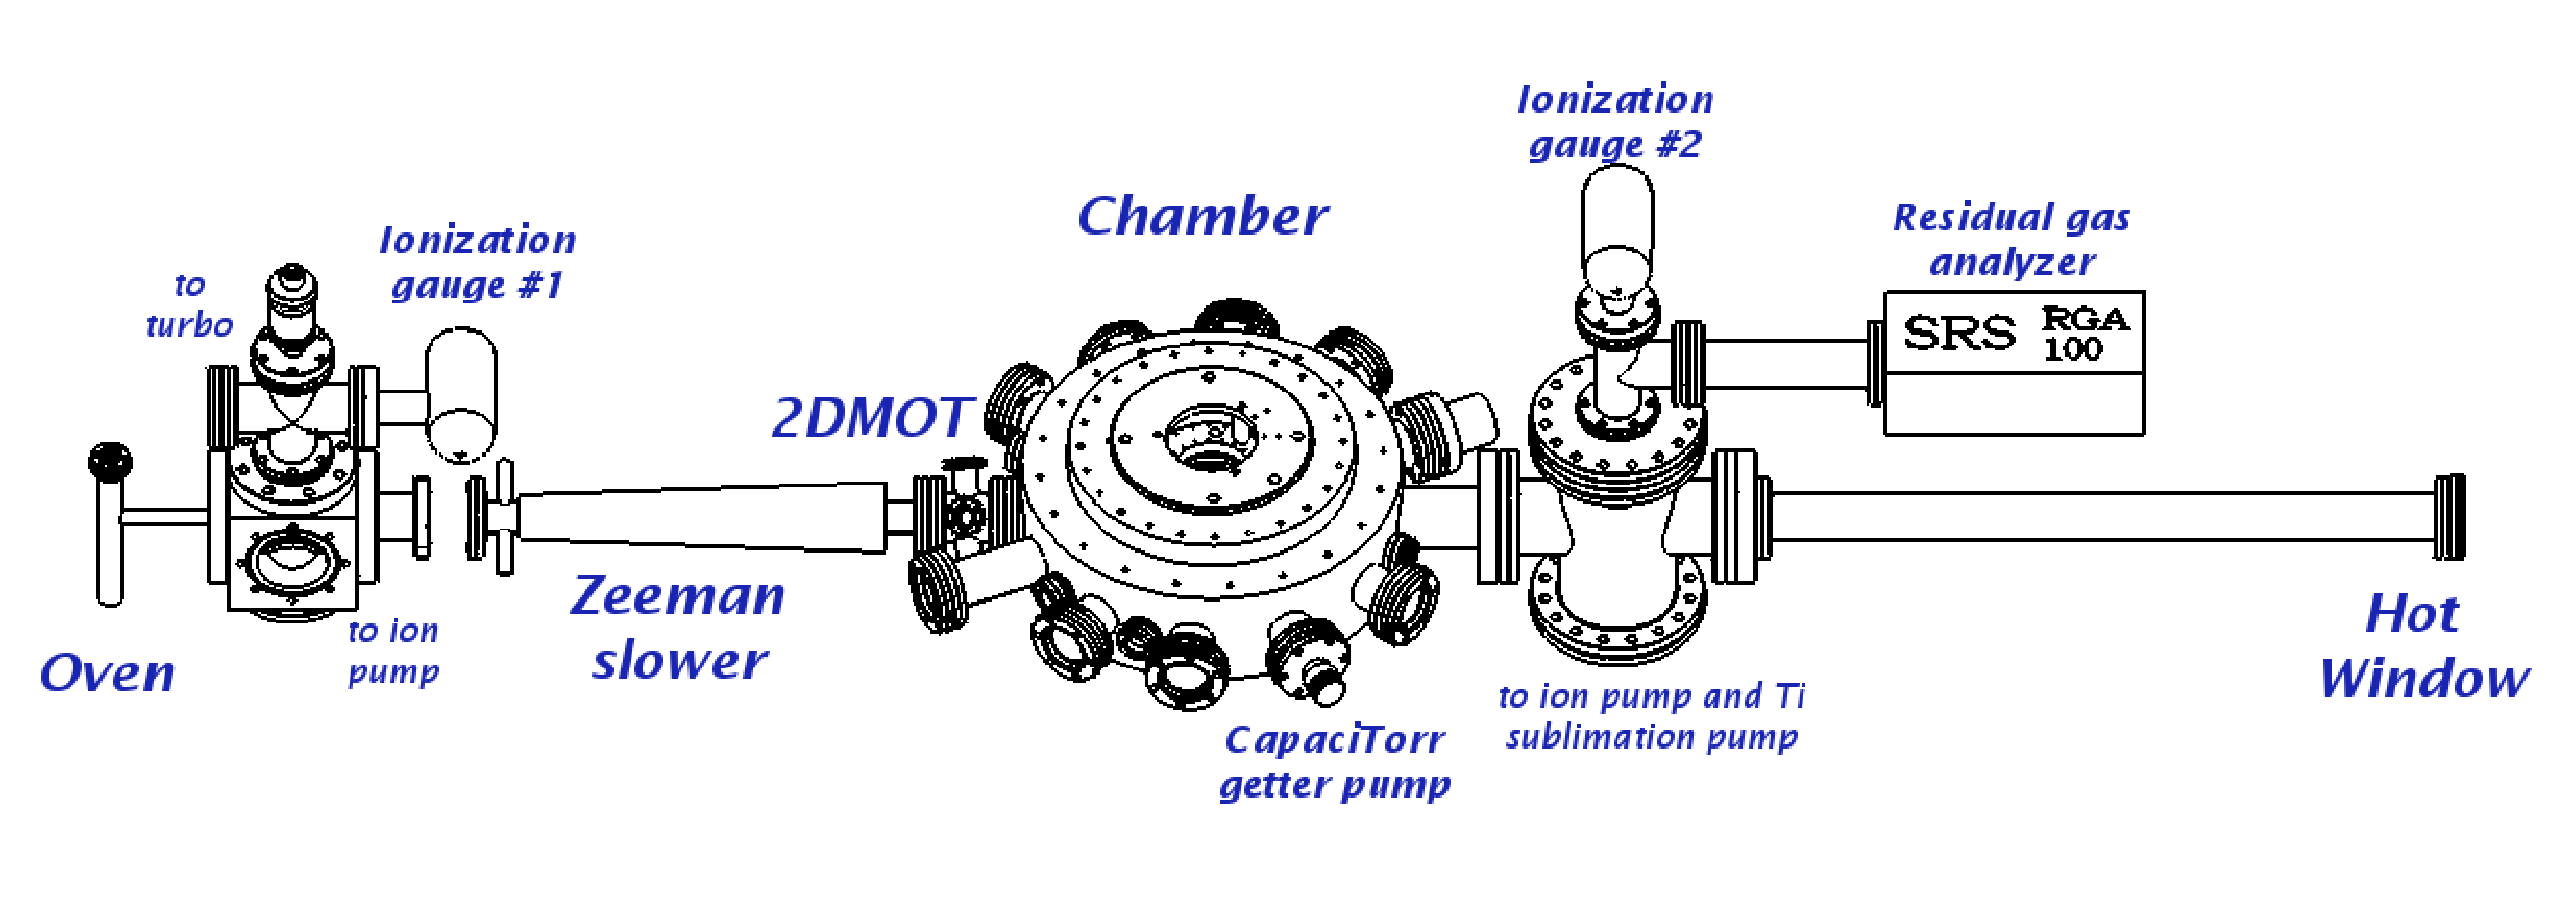
\includegraphics[width=\textwidth]{../masters-figures/vacuum/vacuum02.pdf}
\caption[Apparatus3 vacuum system]{\small Main components of the
vacuum system. } \label{fig:vacuum}
\end{figure}
During operation, the oven section of the vacuum system (see
Fig.~\ref{fig:vacuum}) is heated to 450$^{\circ}$C to produce a collimated beam
of lithium atoms.  The Zeeman slower (described later in
Sec.~\ref{subsec:zeemanslower}) is constructed with a narrow tube and provides
a low conductance (0.5~L/s) that can help maintain 
%up to a factor of 10
a pressure differential between the oven and the main chamber sections.  The
pressure\footnote{Measured with Bayard-Alpert type ionization gauge (Varian
Type 571) labeled \#1 in Fig.~\ref{fig:vacuum}} in the oven section is $4\times
10^{-9}$~Torr, and in the chamber section\footnote{Measured with ion gauge \#2}
is $<5\times10^{-10}$~Torr.   

Lithium atoms that are not captured by the MOT eventually hit a sapphire window
at the far end of the setup, which we refer to as the `hot window' because it
is heated up to around 290$^{\circ}$C to avoid coating it with the lithium
metal.  The long tube between the chamber and the hot window serves a
differential pumping purpose; the tube inside is lined with a helical strip of
non-evaporable getter material\footnote{SAES St 707/CTAM/30D, 30~mm wide
strip.}.

The vacuum is maintained by two ion pumps and a non-evaporable getter pump.  A
VacIon Plus Starcell (150~L/s) from Varian vacuum technologies is connected to
the cross between the chamber and the hot window sections.   A titanium
sublimation cartridge is attached to this pump.  A
smaller Vacion Plus Starcell (55~L/s) is connected to the cube on the oven
section.  A CapaciTorr B200 getter pump (90~L/s for H$_{2}$) is attached
directly to one of the chamber viewports.   Due to the close proximity of this
getter pump to the atoms (8~cm) we expect the background pressure to be lower
in the center of the chamber than the $5\times10^{-10}$~Torr measured with ion
gauge \#2.



%########################################
\section{671 nm laser cooling system}
%########################################


For the Zeeman slower, 2DMOT and MOT we perform laser cooling using the \red\
transition in \li\ (see level diagram in Fig.~\ref{fig:671levels}) which has a
wavelength of 671~nm.    The light is produced in a separate optical table and
transferred to the apparatus table via optical fibers.  In this section we give
a description of the different parts of the 671~nm laser cooling system.  

%On the apparatus table, the MOT light is split into
%six beams and the correct circular polarizations are set.  In this section I
%describe the laser system used to produce the light for the MOT and the Zeeman
%slower, and also give technical information about our Zeeman slower.  Details
%about the operation parameters and characteristics of the MOT are deferred to
%Chapter~\ref{ch:uvmot}.


%----------------------------------------
\subsection{Laser system}
%----------------------------------------

\begin{figure} \centering
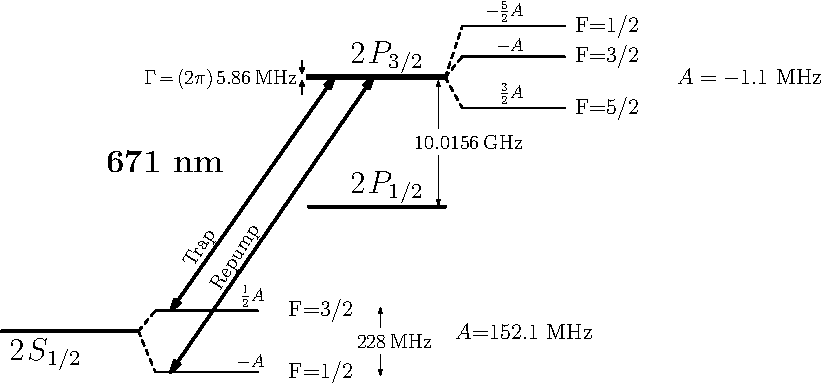
\includegraphics[width=0.85\textwidth]{../masters-figures/levels/671-levels/lithium.pdf}
\caption[Lithium-6 energy level diagram]{\small Energy level diagram showing
transitions relevant for laser cooling \li using the \red transition. }
\label{fig:671levels} \end{figure} 

Efficient laser cooling relies on continuous scattering of photons by the atom.
To avoid optical pumping to a dark hyperfine ground state we use two
frequencies of light, tuned to the $\twos{1/2}\cm\f{3/2}$ and
$\twos{1/2}\cm\f{1/2}$ states.  We refer to these as trap and repump,
respectively, as shown in Fig.~\ref{fig:671levels}. 

%  In a magneto-optical trap, a lithium atom,
%see Fig.~\ref{fig:671levels}, that absorbs a photon on the
%$\twos{1/2}\cm\f{3/2}\rightarrow\twop{3/2}$ transition, referred to as the
%trapping transition, can decay to the
%$\twos{1/2}\cm\f{1/2}$ state.  To maintain the continuous scattering of photons, a
%second frequency that is tuned to the
%$\twos{1/2}\cm\f{1/2}\rightarrow\twop{3/2}$ transition is required; we refer to
%this transition as the repumping transition.  The probability of going to a
%dark state is higher in lithium than in other alkalis such as rubidium, cesium,
%or sodium  because the hyperfine structure of the excited state is unresolved,
%$\Gamma\approx 5|A|$. 

%\begin{sidewaysfigure} \centering
%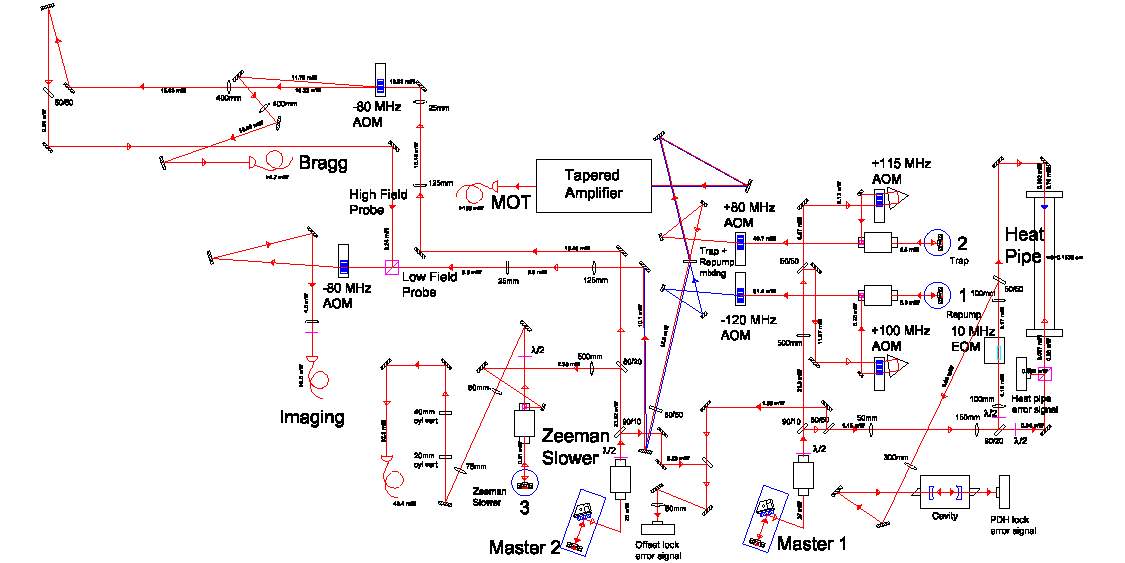
\includegraphics[width=1.\textwidth]{../masters-figures/671setup/671setup(v4).pdf}
%\vspace{1cm} \par \caption[671 nm laser system]{\small Intended for the in
%house reader, this figure shows the layout of the Apparatus3 671 nm laser
%system.  Benchmark powers are indicated on the figure.  } \label{fig:671system}
%\end{sidewaysfigure} 

The laser system that is used to produce the trapping and repumping MOT light,
as well as the Zeeman slower and imaging probe light, was described in detail
in my Master's thesis~\cite{DuarteMs}.    We have two home-built extended
cavity diode lasers, which we refer to as MOT~Master and ZS~Master. The
MOT~Master is stabilized to the $\twos{1/2}\cm\f{3/2}\rightarrow\twop{3/2}$
transition via saturated absorption spectroscopy and the ZS~Master is offset
locked (red detuned) to the MOT~Master using the side-of-filter
technique~\cite{SoftLock2004}.  

\subsubsection{MOT~Master} 

Light from the MOT~Master is split up for producing the trap and repump
frequencies; each path is passed through a double-pass acousto-optic modulator
(AOM) and injection-locks a slave laser diode for amplification.  The light
from the trap and repump slaves is overlapped on a beamsplitter before
injecting a tapered amplifier.  The output from the tapered amplifier is fiber
coupled to the apparatus table.  After passing through an AOM and splitting ten
percent of the light for the 2DMOT, we can get as much as 90 mW of power for
the MOT.   Due to the small splitting between trap and repump frequencies, 22
mW of light are produced by the tapered amplifier in unwanted sidebands at
\mbox{$f_{\mathrm{trap}}-228\,\mathrm{MHz}$} and
\mbox{$f_{\mathrm{repump}}+228\,\mathrm{MHz}$}~\cite{Ferrari1999}. This results
in a net 53~mW of trapping light and 16~mW of repumping light that are
dedicated to the MOT.  

\subsubsection{ZS~Master}
 
Light from the ZS~Master is split up into two paths.  The first path is used as
the probe light in Bragg scattering experiments. It is passed through AOMs for
power control and switching purposes and coupled into an optical fiber.
Approximately 5 mW are available for the experiment at the output end.  The
second path is used to inject a slave laser diode for amplification.  The
output of the slave passes through an AOM, which selects whether the light is
used for Zeeman slowing or imaging.  The zeroth order of the AOM is used for
Zeeman slowing and the 1st order is used as the imaging probe.   Approximately
30~mW (20~mW)  of light are available for Zeeman slowing (imaging) after the
light is coupled into an optical fiber.    

%Besides the loss of power we have not observed negative
%effects in the operation of the MOT from the presence of the sideband
%frequencies created by the tapered amplifier.
%
%The ZS~Master is used to produce the Zeeman slower light and the imaging probe.
%Light from the ECDL is  split into two paths:  the first path injects a slave to
%produce the Zeeman slower light, the second path is diverted to the imaging
%setup.   The light from the Zeeman slower slave is coupled to an optical fiber
%to be transferred to the apparatus table.   Light that goes to the imaging
%setup is passed through an AOM and coupled to a fiber to be used as the probe
%light for atoms at high magnetic field.   
%
%\begin{figure} \centering
%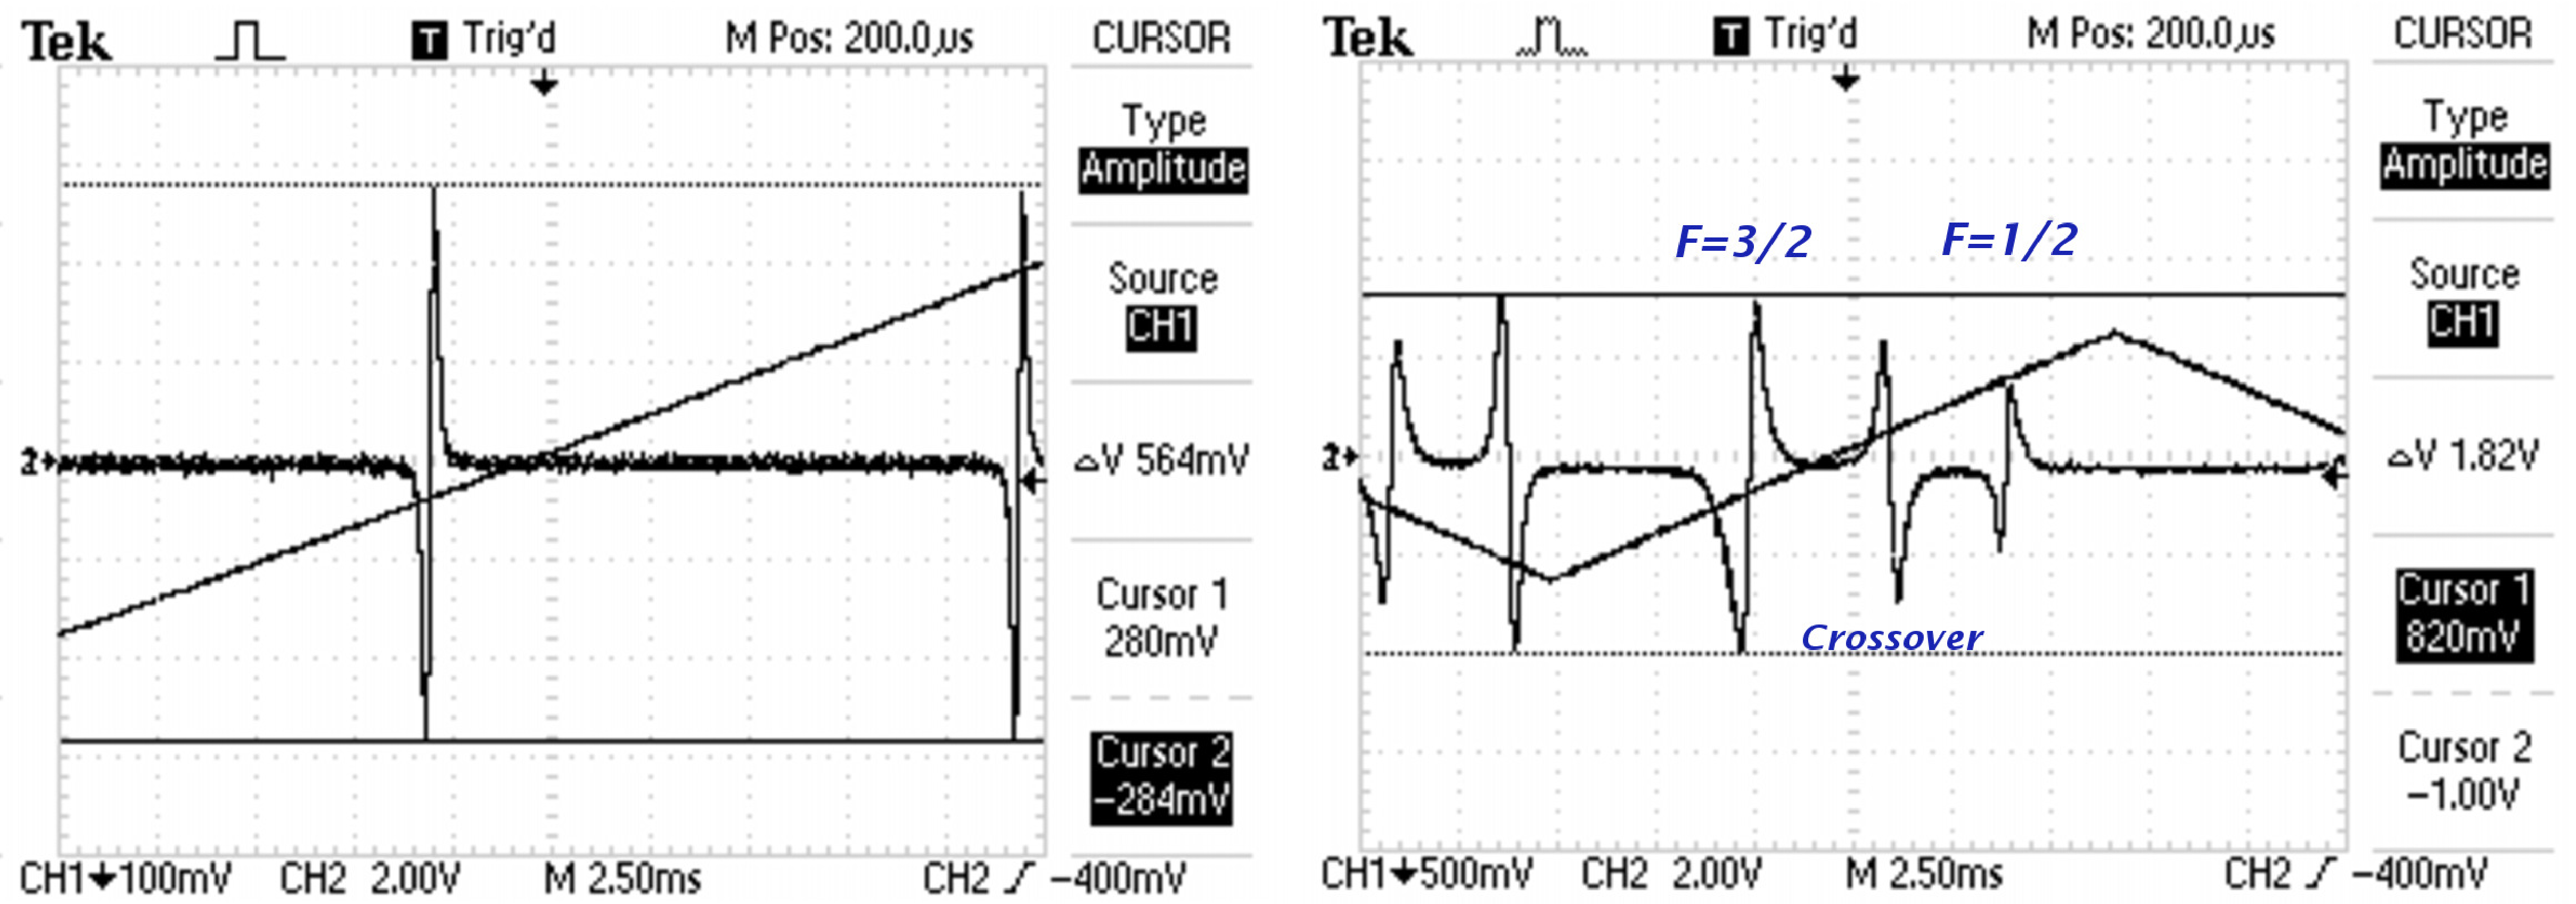
\includegraphics[width=0.95\textwidth]{../masters-figures/671setup/MotMaster.pdf}
%\caption[Lock error signals for  671 nm MOT~Master]{\small The MOT~Master is
%stabilized to the error signal from a Fabry-Perot cavity (left). The cavity is
%stabilized using a saturated absorption spectroscopy error signal obtained from
%a lithium heat pipe.  To obtain both of the error signals shown in this figure
%the Pound-Drever-Hall (PDH) technique is used, where the necessary sidebands
%are produced by phase modulation with an electro-optic modulator at 13 MHz. }
%\label{fig:motmaster} \end{figure}
%
%\begin{figure} \centering
%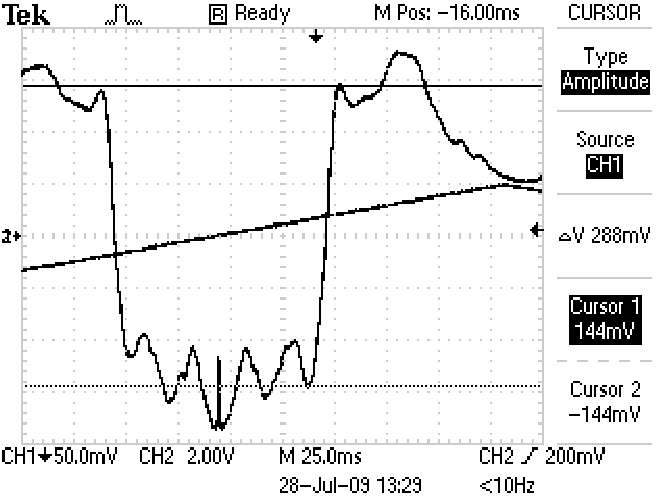
\includegraphics[width=0.475\textwidth]{../masters-figures/671setup/offsetlock.pdf}
%\caption[Side of filter lock error signal for 671 nm ZS~Master]{\small The
%ZS~Master is stabilized using an error signal obtained using the side-of-filter
%technique.   The zero crossing of the error signal is determined by the
%frequency of a local oscillator which can be tuned.  In our setup we can tune
%ZS~Master from -400 MHz to -1500 MHz with respect to  MOT~Master.  }
%\label{fig:zsmaster} \end{figure}

	
%----------------------------------------
\subsection{Zeeman slower}
\label{subsec:zeemanslower}
%----------------------------------------
The Zeeman slower reduces the speed of atoms coming out of the oven to less
than the capture velocity of our MOT, $v_{\mathrm{c}}\simeq 5\Gamma/k = 20$
m/s, where $5\Gamma$ is the red detuning from resonance at which we operate the
MOT during loading. The Zeeman slower works by using red detuned laser light
propagating opposite to the lithium atomic beam.  Due to the Doppler shift, the
laser light is resonant with atoms coming out of the oven, and via repeated
photon scattering can produce a maximum deceleration given by $a_{\mathrm{max}}
= \frac{h\Gamma}{2\lambda m}$.  As the atoms get slowed they shift out of
resonance, but the spatially dependent magnetic field of the Zeeman slower
shifts the transition to the red keeping the atoms resonant with the light as
they travel through the slower.

The Zeeman slower operates on the $\sigma^{-}$  transition between the
$\twos{1/2}\cm\f{3/2}\cm\mf{-3/2}$ and $\twop{3/2}\cm\f{5/2}\mf{-5/2}$ levels,
shown in red in Fig.~\ref{fig:zeemanlevels}. An advantage of choosing this
transition is that it is a cycling transition even at moderate magnetic fields.
This eliminates the need for using repumping light in the Zeeman slower.  
\begin{figure}
\centering
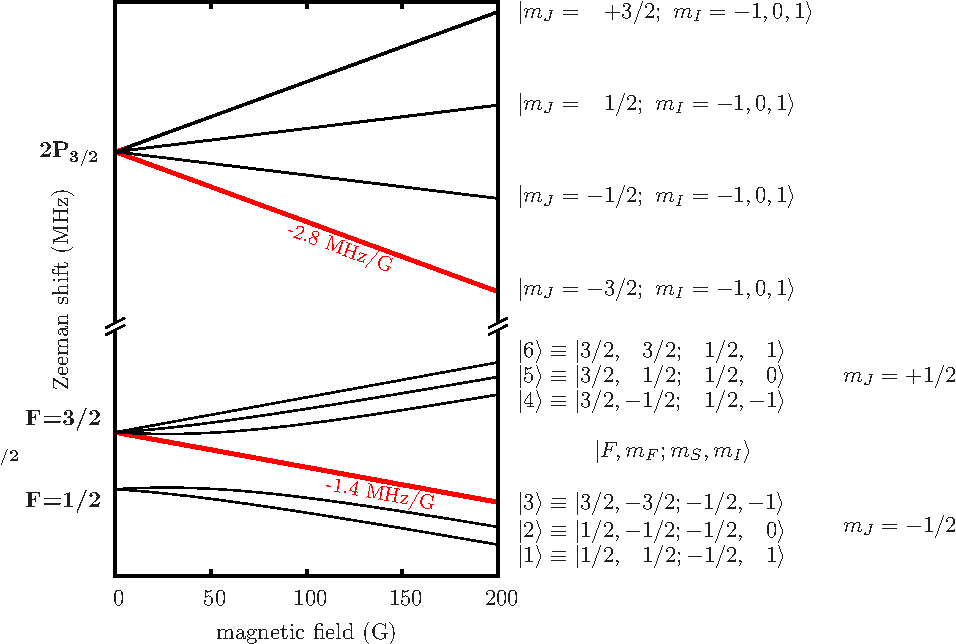
\includegraphics[width=1.0\textwidth]{../masters-figures/levels/zeeman_revised/01eps.pdf}
\caption[Levels of \li in a magnetic field. ]{\small Energy level diagram of
\li in a magnetic field.   The red lines show the levels used in the Zeeman
slower.  } \label{fig:zeemanlevels} 
\end{figure} 
We use a detuning of 1312~MHz, and a magnetic field profile given by \[ B_{z} =
B_{0}(1-\sqrt{1-z/L}) \] where $B_{0}\approx800$~G and $L=34.5$~cm.   



%----------------------------------------
\subsection{2DMOT and MOT}
%----------------------------------------
The 671 nm MOT is loaded from a Zeeman slower plus a 2DMOT. The 2DMOT is at the
output of the Zeeman slower and helps collimate the slow thermal beam of atoms
before it reaches the MOT.   The 2DMOT consists of a quadrupole field with two
pairs of counter-propagating beams which lie on a plane almost normal to the
direction of propagation of the atomic beam.   In our setup, the atomic beam is
offset from the center of the chamber by $\sim1\,$cm, and the angle of the
2DMOT is such that the slowed atoms from the Zeeman slower will be redirected
towards the MOT, located at the center of the chamber (see
Fig.~\ref{fig:apparatus-schem}). 
\begin{figure}
\centering
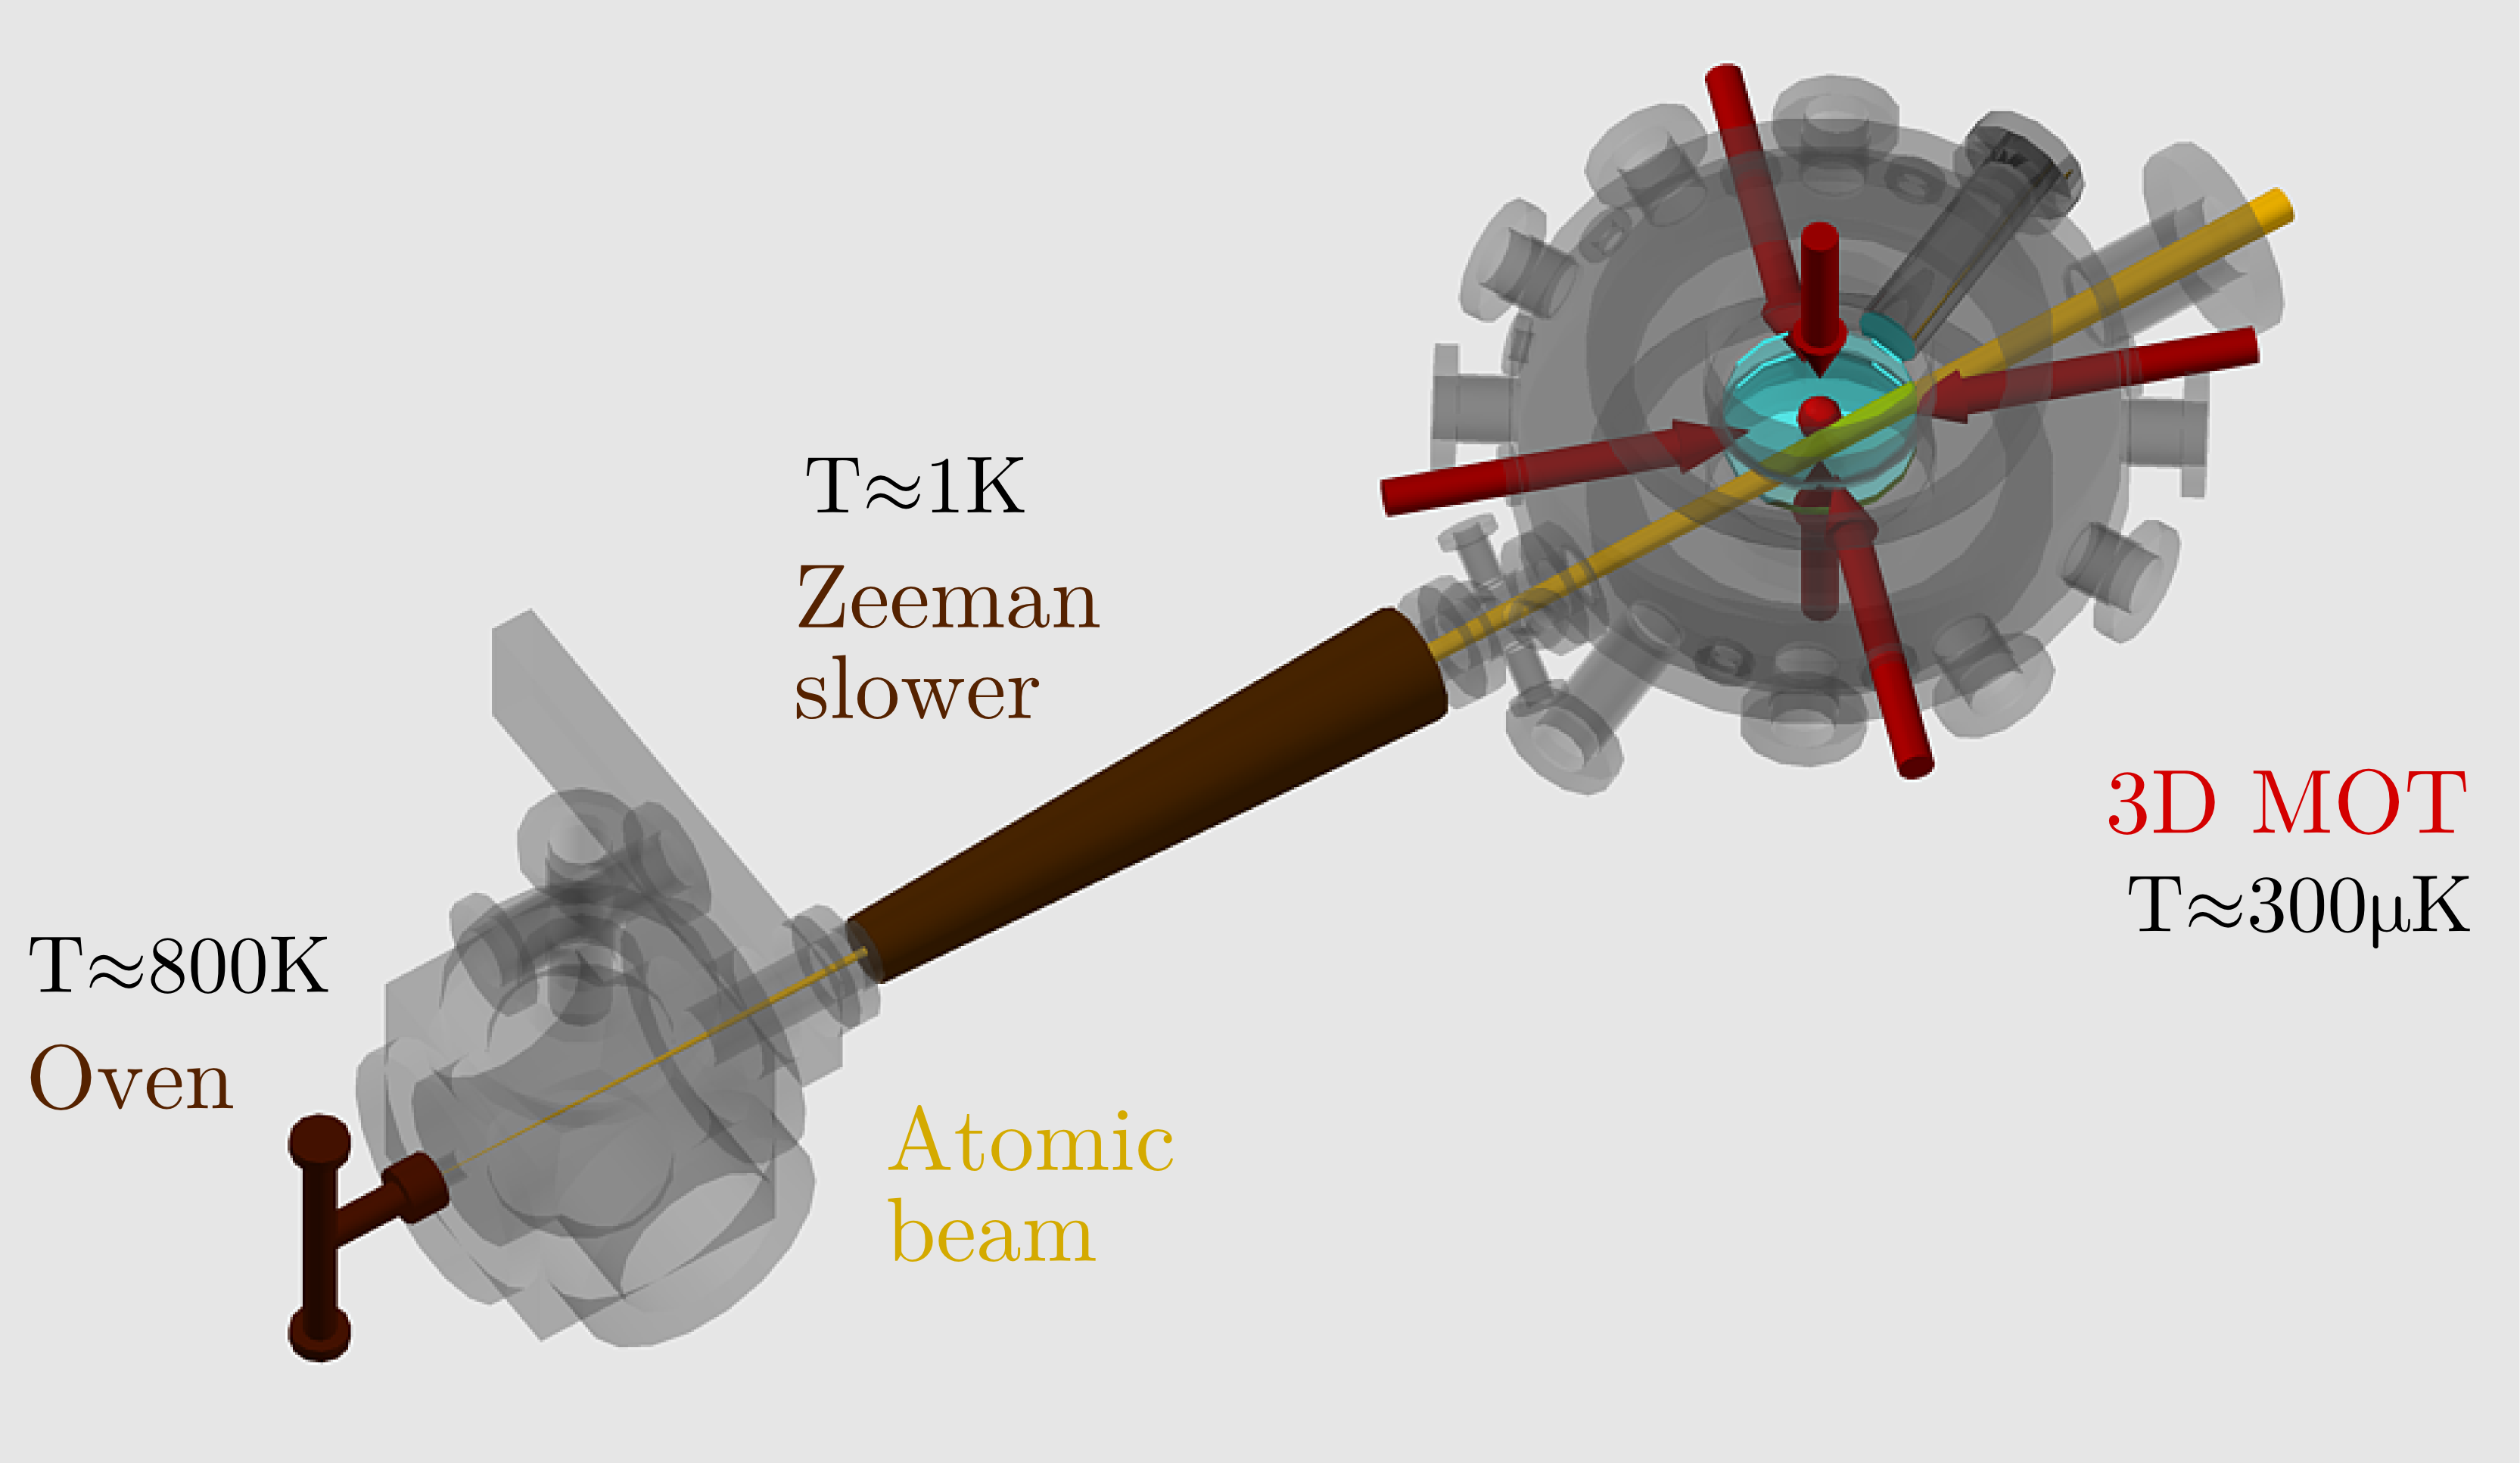
\includegraphics[width=0.8\textwidth]{../masters-figures/apparatus-schem.png}
\caption[Apparatus schematic ]{\small Schematic of apparatus showing the oven,
Zeeman slower and 3DMOT.  The 2DMOT beams (not shown) enter the setup on the
small 4-way cross located between the slower and the main chamber. Notice that
the atomic beam is slightly offset from the center of the chamber. }
\label{fig:apparatus-schem} 
\end{figure} 

In 5~s we load 1.4$\times10^{9}$ atoms in the MOT at a temperature of
$\sim$780~$\mu$K.  After loading, we shutter the Zeeman slower laser using a
hard disk drive shutter~\cite{HardDriveShutter2007}.   At this point we proceed
to cool and compress the 671 nm MOT by  reducing the intensity and detuning of
the the cooling and repumping light, and increasing the magnetic field gradient
to the values shown as CMOT on Table.~\ref{tab:cmot}.
\begin{table}

\centering
\scalebox{1.0}{
\begin{tabular}{l|cc|c}
 &  MOT & CMOT & unit\\
\hline  \hline \noalign{\smallskip}
Trap intensity per beam   & 1.26 & 0.034 & $\isat^{2P}$ \\
Trap detuning   & -33 & -12 & MHz\\
Repump intensity per beam & 0.36 & 0.007 & $\isat^{2P}$ \\
Repump detuning & -25.2 & -17 & MHz\\
$dB_{z}/dz$  & 22.6 & 26.1  & G/cm \\ 
\hline \noalign{\smallskip}
Number & 1.5  & 1 & $10^{9}$\\
$1/e$ radius & 0.22 & 0.18  & cm\\
Peak density  & 2.39 & 3.40 & $10^{10}$cm$^{-3}$\\ 
Temperature & 783 & 288 & $\mu$K\\
Phase space density &  3.9$\times 10^{-7}$ & 2.5$\times 10^{-6}$ & -  
\end{tabular}}
\caption[671 nm MOT cooling and compression]{\small Comparison between the
settings used for loading the 671 nm MOT and the settings after cooling and
compressing (CMOT).   $\isat^{2P}=5.1\,\mathrm{mW/cm^{2}}$ is the saturation
intensity of the 671~nm transition. For cooling and compressing, first the
field gradient is increased in 40 ms, then after a wait of 40 ms the intensity
and detuning of the beams are ramped linearly to their final values in 1 ms.
The phase space density is defined as $n_{0}\lambda_{T}^{3}$ where $n_{0}$ is
the peak density and $\lambda_{T}=\frac{h}{(2\pi m \kb T)^{1/2}}$  is the
thermal de Broglie wavelength. } 
\label{tab:cmot}
\end{table}
 We take time-of-flight images of
the MOT and the CMOT, and infer their temperatures by fitting the cloud sizes
to a ballistic expansion as shown in Fig.~\ref{fig:cmotexp}.   
\begin{figure} \hspace{0.16\textwidth}
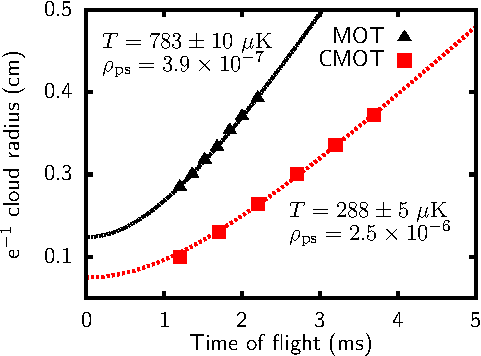
\includegraphics[width=0.58\textwidth]{../masters-figures/323mot/tofexpansion-00/tofeps-SS.pdf}
\caption[671 nm cooled and compressed MOT]{\small  Time-of-flight expansion of
atoms released from the 671 nm MOT right after loading (black triangles) and after
cooling and compressing (red squares). The points represent the $1/e$ width of
Gaussian fits to the spatial profile of the freely expanding clouds.  The lines
are fits to ballistic expansions. $\rho_{\mathrm{ps}}$ stands for phase-space density. } \label{fig:cmotexp} \end{figure}



%########################################
\section{323 nm laser cooling system}
%########################################

Atoms from the 671~nm MOT are transferred to the 323~nm UVMOT, where owing to
the smaller Doppler temperature limit,  lower temperatures can be achieved (see
Fig.~\ref{fig:323levels}).   The Doppler temperature limit, $T_{D}$, of laser
cooling is set by the linewidth of the excited state.  The \uv\ transition
being narrower that the \red\ allows for a lower value of $T_{D}$.  Furthermore
the wavelength of the transition being smaller results in a smaller optical
scattering cross section, which enables reaching larger densities in the UVMOT,
a feature that is favorable when loading the atoms into an optical dipole
trap~\cite{Duarte2011}. 
\begin{figure} \centering
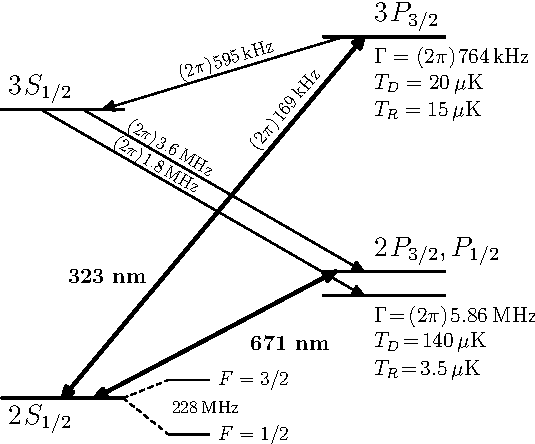
\includegraphics[width=0.65\textwidth]{../masters-figures/levels/323-levels/lithium.pdf}
\caption[Lithium-6 energy level diagram showing the \trep{3/2} state]{\small
Lithium-6 energy level diagram. Lines in bold represent the transitions used to
laser cool atoms. Lighter lines represent decay pathways from the excited
\trep{3/2} state; the decay rates are indicated along the associated paths. On
the right side, beside each excited state we show its linewidth, the associated
Doppler temperature limit ($T_{D}$),  and the recoil temperature limit
($T_{R}$).  }
\label{fig:323levels} \end{figure} 

%----------------------------------------
\subsection{Laser system}
%----------------------------------------

The 323~nm laser system is much simpler than the 671~nm system.  We use a
commercial second harmonic generation (SHG) system from Toptica Photonics to
generate the UV light.  The frequency is stabilized via saturated absorption
spectroscopy, and trapping and repumping frequencies are derived via using
acousto-optic modulators.  The 323~nm system is on the same table as the vacuum
system so we do not use optical fibers,  the light is guided in free space
using mirrors to the final UVMOT configuration.  A schematic of the laser
system is shown in Fig.~\ref{fig:323setupfig}. 
\begin{figure} \centering
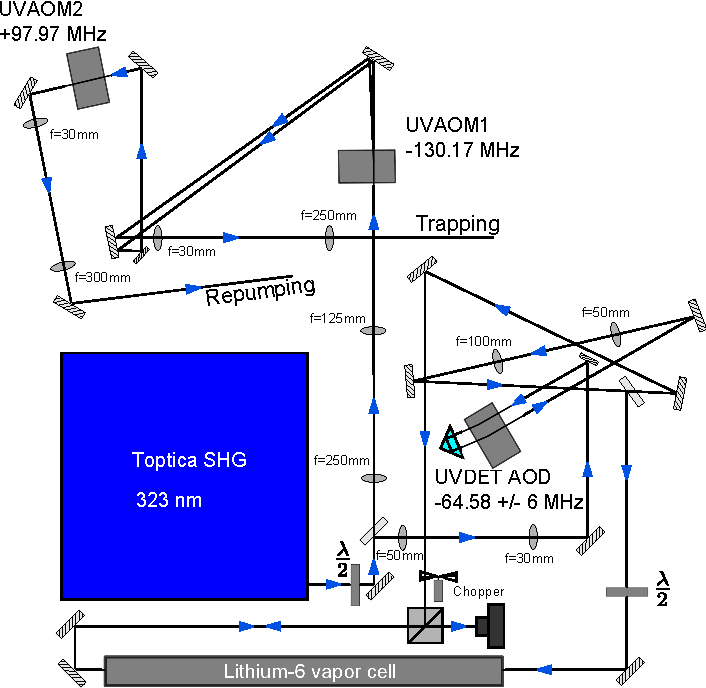
\includegraphics[width=0.7\textwidth]{../masters-figures/323setup/aomsetup/optical_setup.pdf}
\caption[Schematic of modulation transfer spectroscopy]{\small Schematic
showing the optical setup for the 323~nm laser system.   The frequency is
stabilized using a saturated absorption spectroscopy setup~\cite{DuarteMs}.
The light that goes to the experiment is passed through an AOM (labeled
UVAOM1),  the first order is used for trapping and the zeroth order is sent to
a second AOM (labeled UVAOM2) whose first order is used as the repump
frequency.  Trapping and repumping light are combined (not shown) and then
split into six paths for the UVMOT.}
\label{fig:323setupfig}  
\end{figure}


%----------------------------------------
\subsection{UVMOT}
%----------------------------------------

To choose the waist of  the UVMOT beams we had to take into consideration the
available laser power and the transmission losses on the viewports of our
apparatus, which are not anti-reflection coated at
323 nm.  Figure~\ref{fig:012} tabulates the losses at each viewport.
\begin{figure} \begin{minipage}{0.5\linewidth}
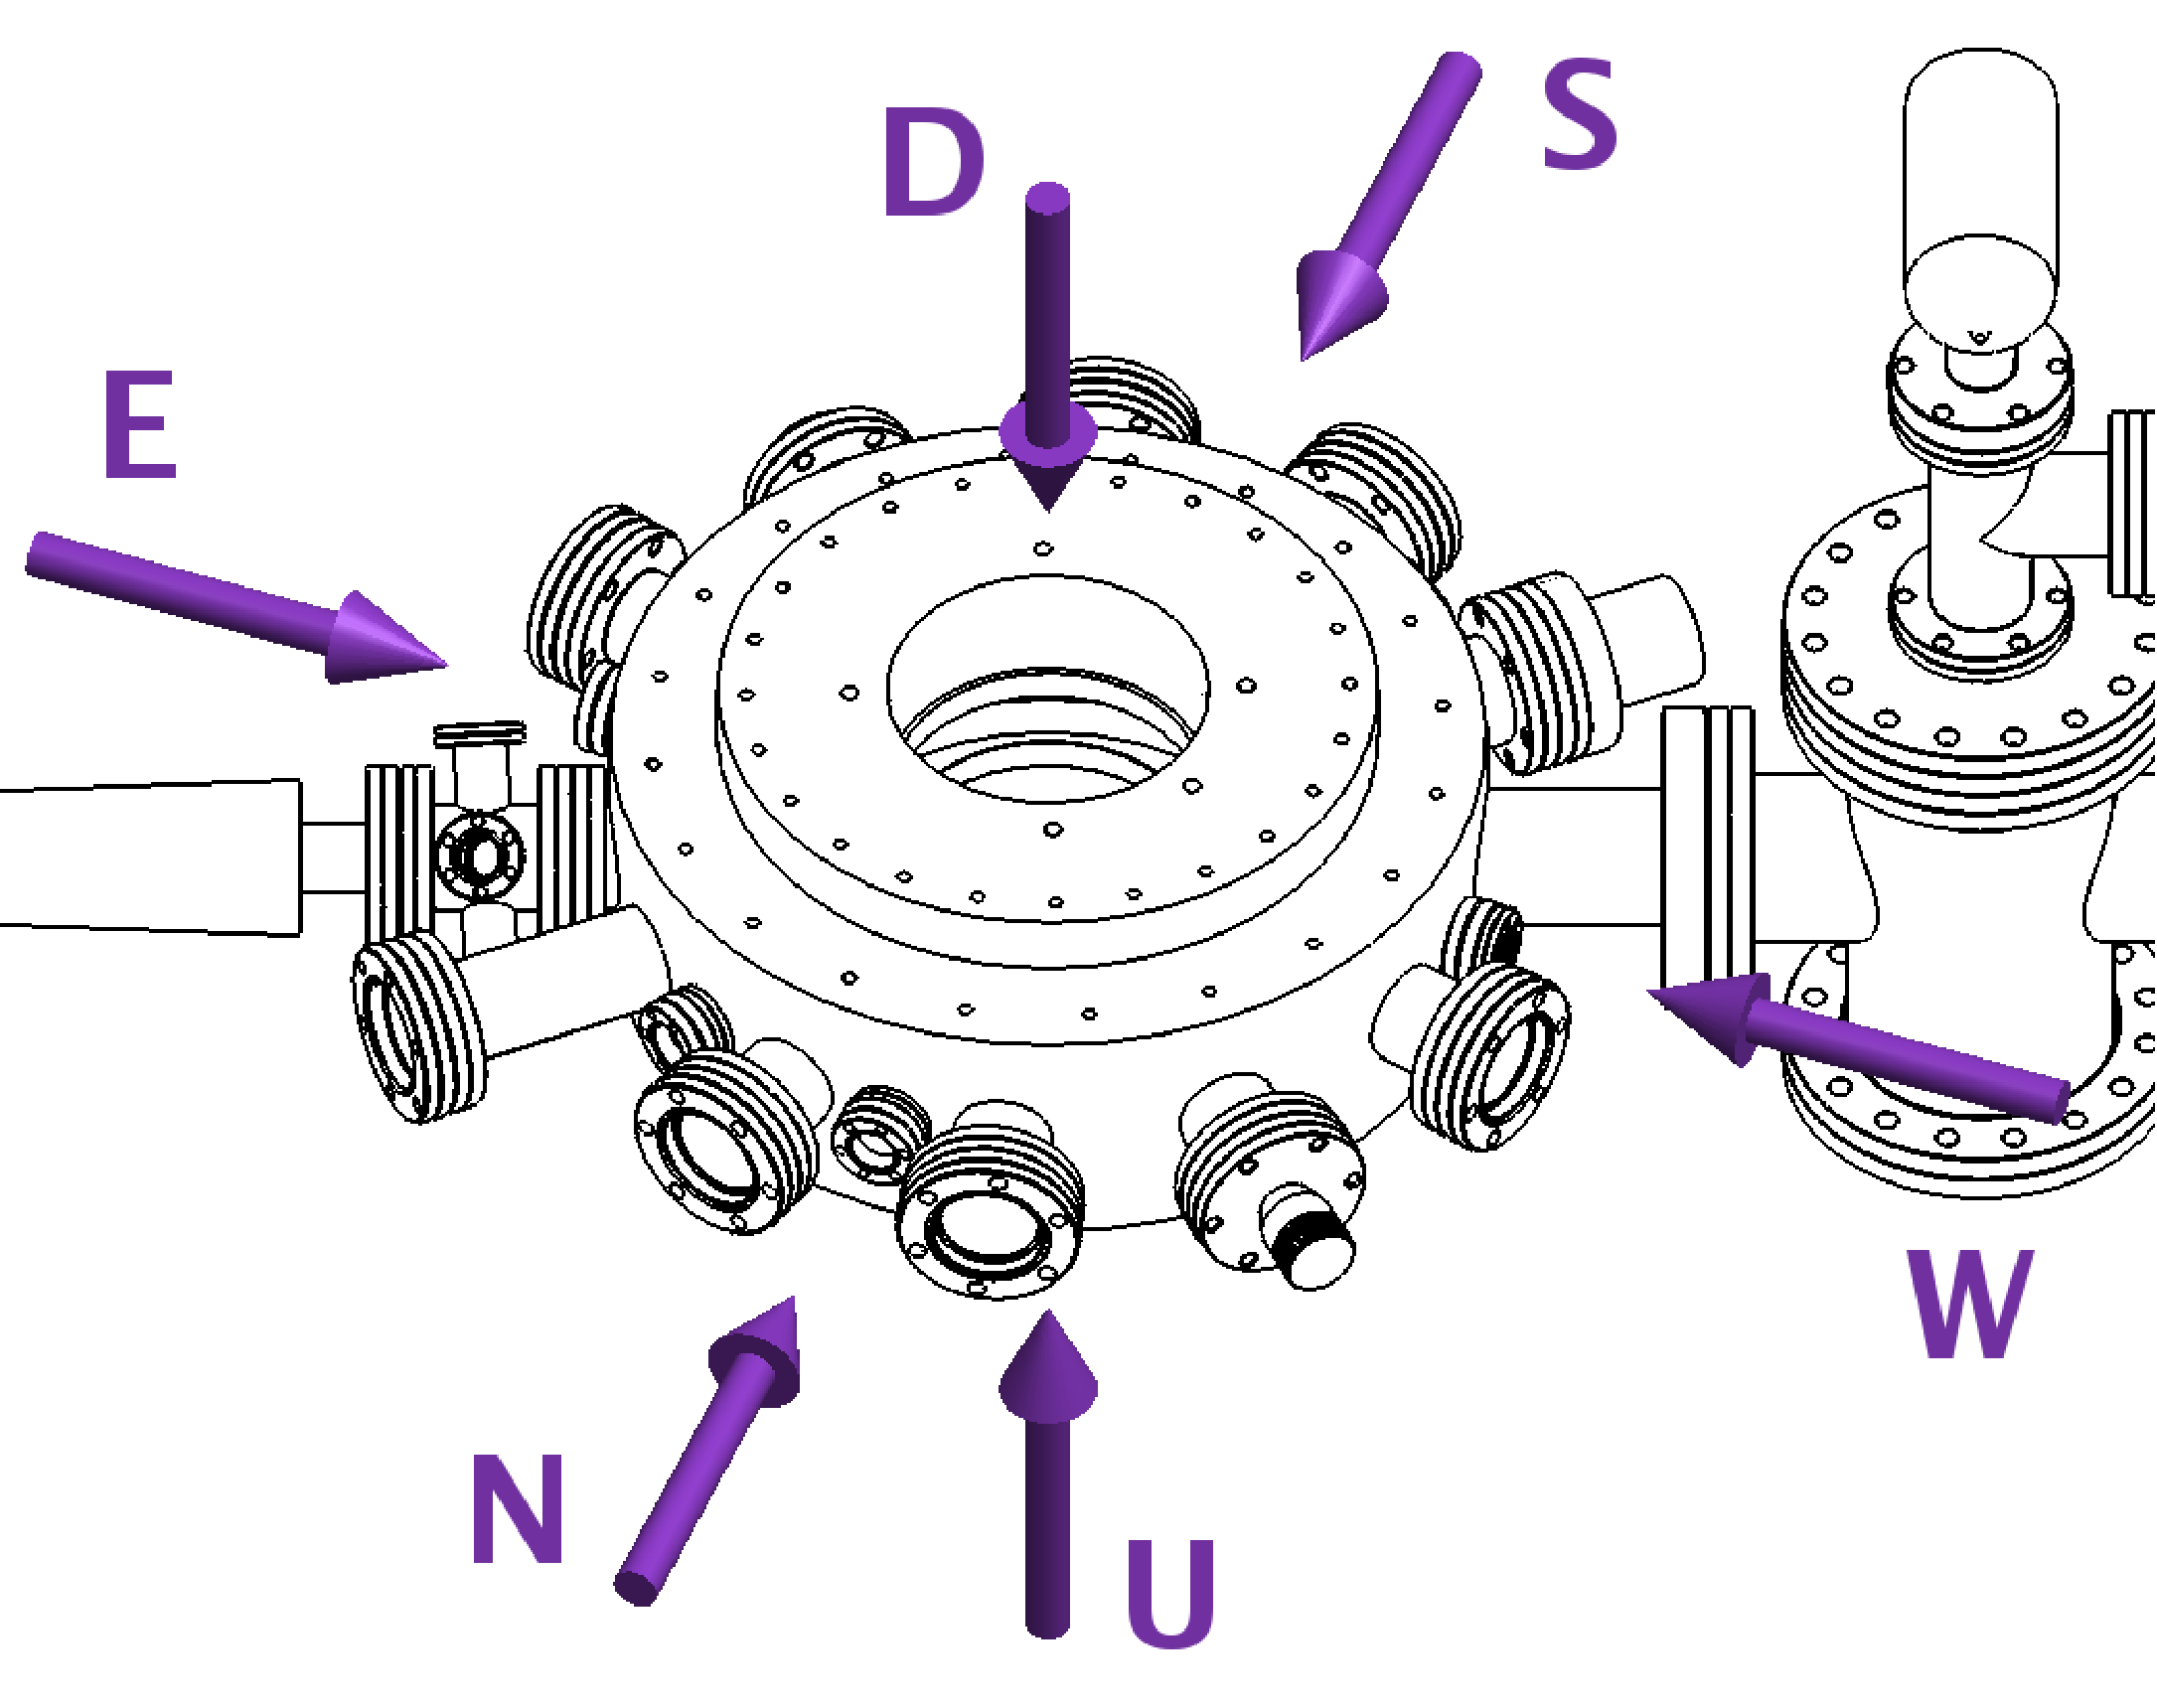
\includegraphics[width=\textwidth]{../masters-figures/323setup/losses/losses.pdf}
\end{minipage} \begin{minipage}{0.5\linewidth} \centering \begin{tabular}{r|c}
& \% Transmission  \\ \hline N & 68 \\ S & 87 \\ E & 75 \\ W & 58 \\ U & 40 \\
D & 40 \\ \end{tabular} \end{minipage} \caption[UVMOT Losses on windows]{\small
This figure shows the percentage transmission of the 323 nm light through the
viewports on our vacuum chamber.  For the side viewports the losses were
accounted for by measuring the power reflected back by the window.  For the top
and bottom viewport it was harder to make this measurement due to restricted
access, so the square root of the transmission through both windows is used. }
\label{fig:012} \end{figure} 
We set up all the beams to have the same intensity at the atoms, thus carefully
taking into account the losses at each window.  This was accomplished by
varying the angle of incidence on dielectric beamsplitters until the desired
power ratios were achieved.  
%Polarization beamsplitter cubes for 323 nm are expensive because they have to
%be optically contacted.  We have observed that the UV light progressively
%damages the cement used in lower priced polarizing beam-splitter cubes.  We
%did keep one polarizing beam-splitter cube (not optically contacted) in our
%setup for doing the first split of the UVMOT beams.  This allows some
%variability in the power balance without having to realign the entire system.
%Currently we loose 14\% of the light on the mentioned cube.  
Considering the losses at the windows and other UV optics, We set the beam waist
of the UVMOT beams to 3.3~mm, which results in an intensity of 1.0$\isat^{3P}$
per beam at an SHG output power of 27.4~mW.  Here $\isat^{3P}=5.9$\,mW/cm$^{2}$
is the saturation intensity of the 323~nm transition.  

The UVMOT uses the same viewports as the 671 nm MOT. All six beams of both
wavelengths are overlapped on dichroic mirrors that transmit 671 nm and reflect
323 nm.  We were lucky to find a long-pass filter (Part Num. NT64-634) from
Edmund Optics that, at very low cost per piece, provides $>99$\% reflection at
323 nm and $>99$\% transmission at 671 nm for both S and P polarizations at a
45$^{\circ}$ angle of incidence.  The UVMOT and red MOT share an axis with the
optical dipole trap (beams $S$ and $N$ on Fig.~\ref{fig:012}).   After the 671
nm and 323 nm are combined, they are overlapped with the optical dipole trap
(1070~nm) or optical lattice (1064~nm) light using a trichroic mirror (Custom
made part from RMI Co.)  that reflects IR and transmits 671~nm and 323~nm.  The
trichroic mirrors have a reflection coefficient  $R>99.5$\% measured at 1064 nm
and 1070 nm, and a transmission coefficient $T=99$\% at 671 nm and $T=90$\% at
323 nm, all measured at a 45$^{\circ}$ angle of incidence.  Also the $U$ and
$D$ beams of the UVMOT share an axis with the optical lattice (1064~nm and
532~nm).  In this case a tetrachroic mirror (Lambda Research Optics) is used to
overlap the wavelengths.  This mirror satisfies $R_{532\,\mathrm{nm}} \approx
0.92$, $R_{1064\,\mathrm{nm}}\approx 0.99$, $T_{671\,\mathrm{nm}}\approx0.92$,
and $T_{323\,\mathrm{nm}}\approx0.86$. 


%----------------------------------------
\subsection{Transfer from MOT to UVMOT}
\label{subsec:mot-uvmot}
%----------------------------------------


The timing diagram for loading the UVMOT from the CMOT is shown
in Fig.~\ref{fig:timingUV}.  The procedure consists of quickly reducing the
magnetic field gradient and turning on the UV light at the same time as the
671~nm light is turned off.  The magnetic field gradient is ramped back up
slowly for compression.  The UV detuning is constant throughout.  The
operating values of the UVMOT are shown in Table~\ref{tab:uvmotUV}, and a
measurement of the temperature is shown in Fig.~\ref{fig:uvtexpUV}. 

\begin{figure} \centering
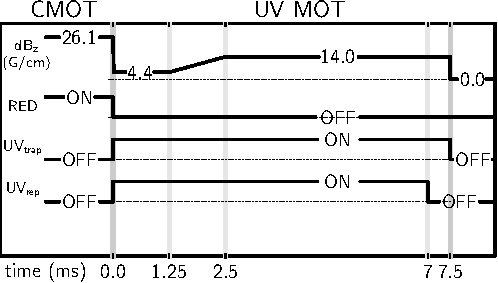
\includegraphics[width=0.5\textwidth]{../masters-figures/323mot/timingdiagram-nodet/timing.pdf}
\caption[UVMOT loading timing diagram]{\small Timing diagram representing the
transfer sequence from the CMOT to the UVMOT. } \label{fig:timingUV}
\end{figure}

\begin{table} \centering 
\scalebox{1.0}{
\begin{tabular}{l|c|c} 
&  UVMOT  & unit\\ 
\hline  \hline \noalign{\smallskip} 
$dB_{z}$ Final & 14 & G/cm \\ 
\hline \noalign{\smallskip}
SHG Output power &  25 & mW \\
UV trap intensity per beam & 1.0 & $\isat^{3P}$ \\
UV repump intensity per beam & 0.1 & $\isat^{3P}$ \\
UV detuning (UVMOT only) & -1.6 & MHz \\
UV detuning (loading to ODT) & -0.6 & MHz \\
\hline \noalign{\smallskip} 
Number & 5.3 & $10^{8}$  \\ 
$1/e$ radius & 0.15  & cm \\ 
Peak density & 2.9  & $10^{10}$\,cm$^{-3}$ \\ 
Temperature & 59 & $\mu$K \\ 
Phase space density &  2.3$\times 10^{-5}$ & - 
\end{tabular}}
\caption[UVMOT settings]{\small UVMOT Settings.
$\isat^{3P}=5.9\,\mathrm{mW/cm^{2}}$ is the saturation intensity of the 323~nm
transition.~\cite{Duarte2011}. The two values shown for the detuning correspond
to optimized number and temperature of the UVMOT (Fig.~\ref{fig:uvtexpUV}), and
optimized number of atoms loaded into the ODT.  More details on loading the ODT
will be given on \S\ref{sec:odtload}. }
\label{tab:uvmotUV} \end{table}

\begin{figure}
\hspace{0.16\textwidth}
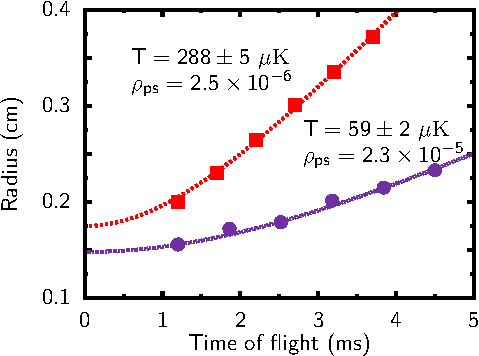
\includegraphics[width=0.58\textwidth]{../masters-figures/323mot/tofexpansion/tofeps.pdf}
\caption[CMOT and UVMOT time-of-flight expansion]{\small Time-of-flight
expansion of the CMOT (red squares) and the UVMOT  (violet circles).  The
points represent the $1/e$ width of Gaussian fits to the spatial profile of the
freely expanding clouds.  The lines are fit to ballistic expansions.
$\rho_{\mathrm{ps}}$ stands for phase-space density.}
\label{fig:uvtexpUV} \end{figure} 



%########################################
\section{Optical dipole trap}
%########################################

We load the atoms from the UVMOT into the optical dipole trap (ODT), where we
evaporatively cool them to degeneracy. The light for the ODT is provided by a
broadband fiber laser operating at 1070~nm with an output power of 50~W.  Two
beams with orthogonal polarizations cross at an angle of 15$^{\circ}$ to form a
crossed-beam trap. The resulting potential resembles an elongated ellipsoid, as
shown in Fig.~\ref{fig:odt-cartoon}. 
\begin{figure} \centering
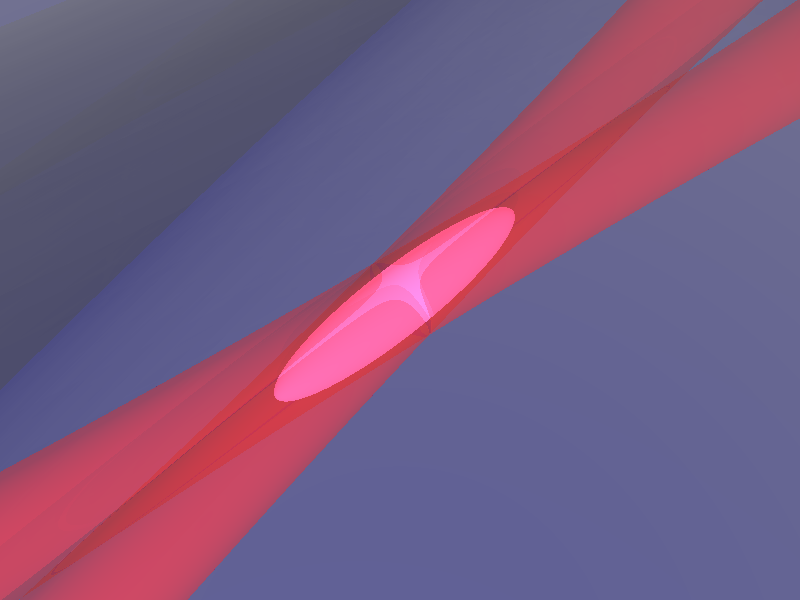
\includegraphics[width=0.4\textwidth]{../masters-figures/odt/15deg-crossbeam.png}
\caption[Optical dipole trap]{\small Illustration of the potential created by
the crossed-beam optical dipole trap.  } \label{fig:odt-cartoon}
\end{figure}

The ODT beams are cylindrically symmetric and focused to a waist of
$\sim70~\mu$m.  For the purposes of tuning the potential to optimize the number
of atoms loaded, the lens labeled $F$ in Fig.~\ref{fig:odtsetup} is positioned
on a translation stage.  Moving this lens along the beam path has a strong
handle on the waist of the ODT beams, and thus affects the depth and volume of
the trap strongly.  
\begin{figure} \centering
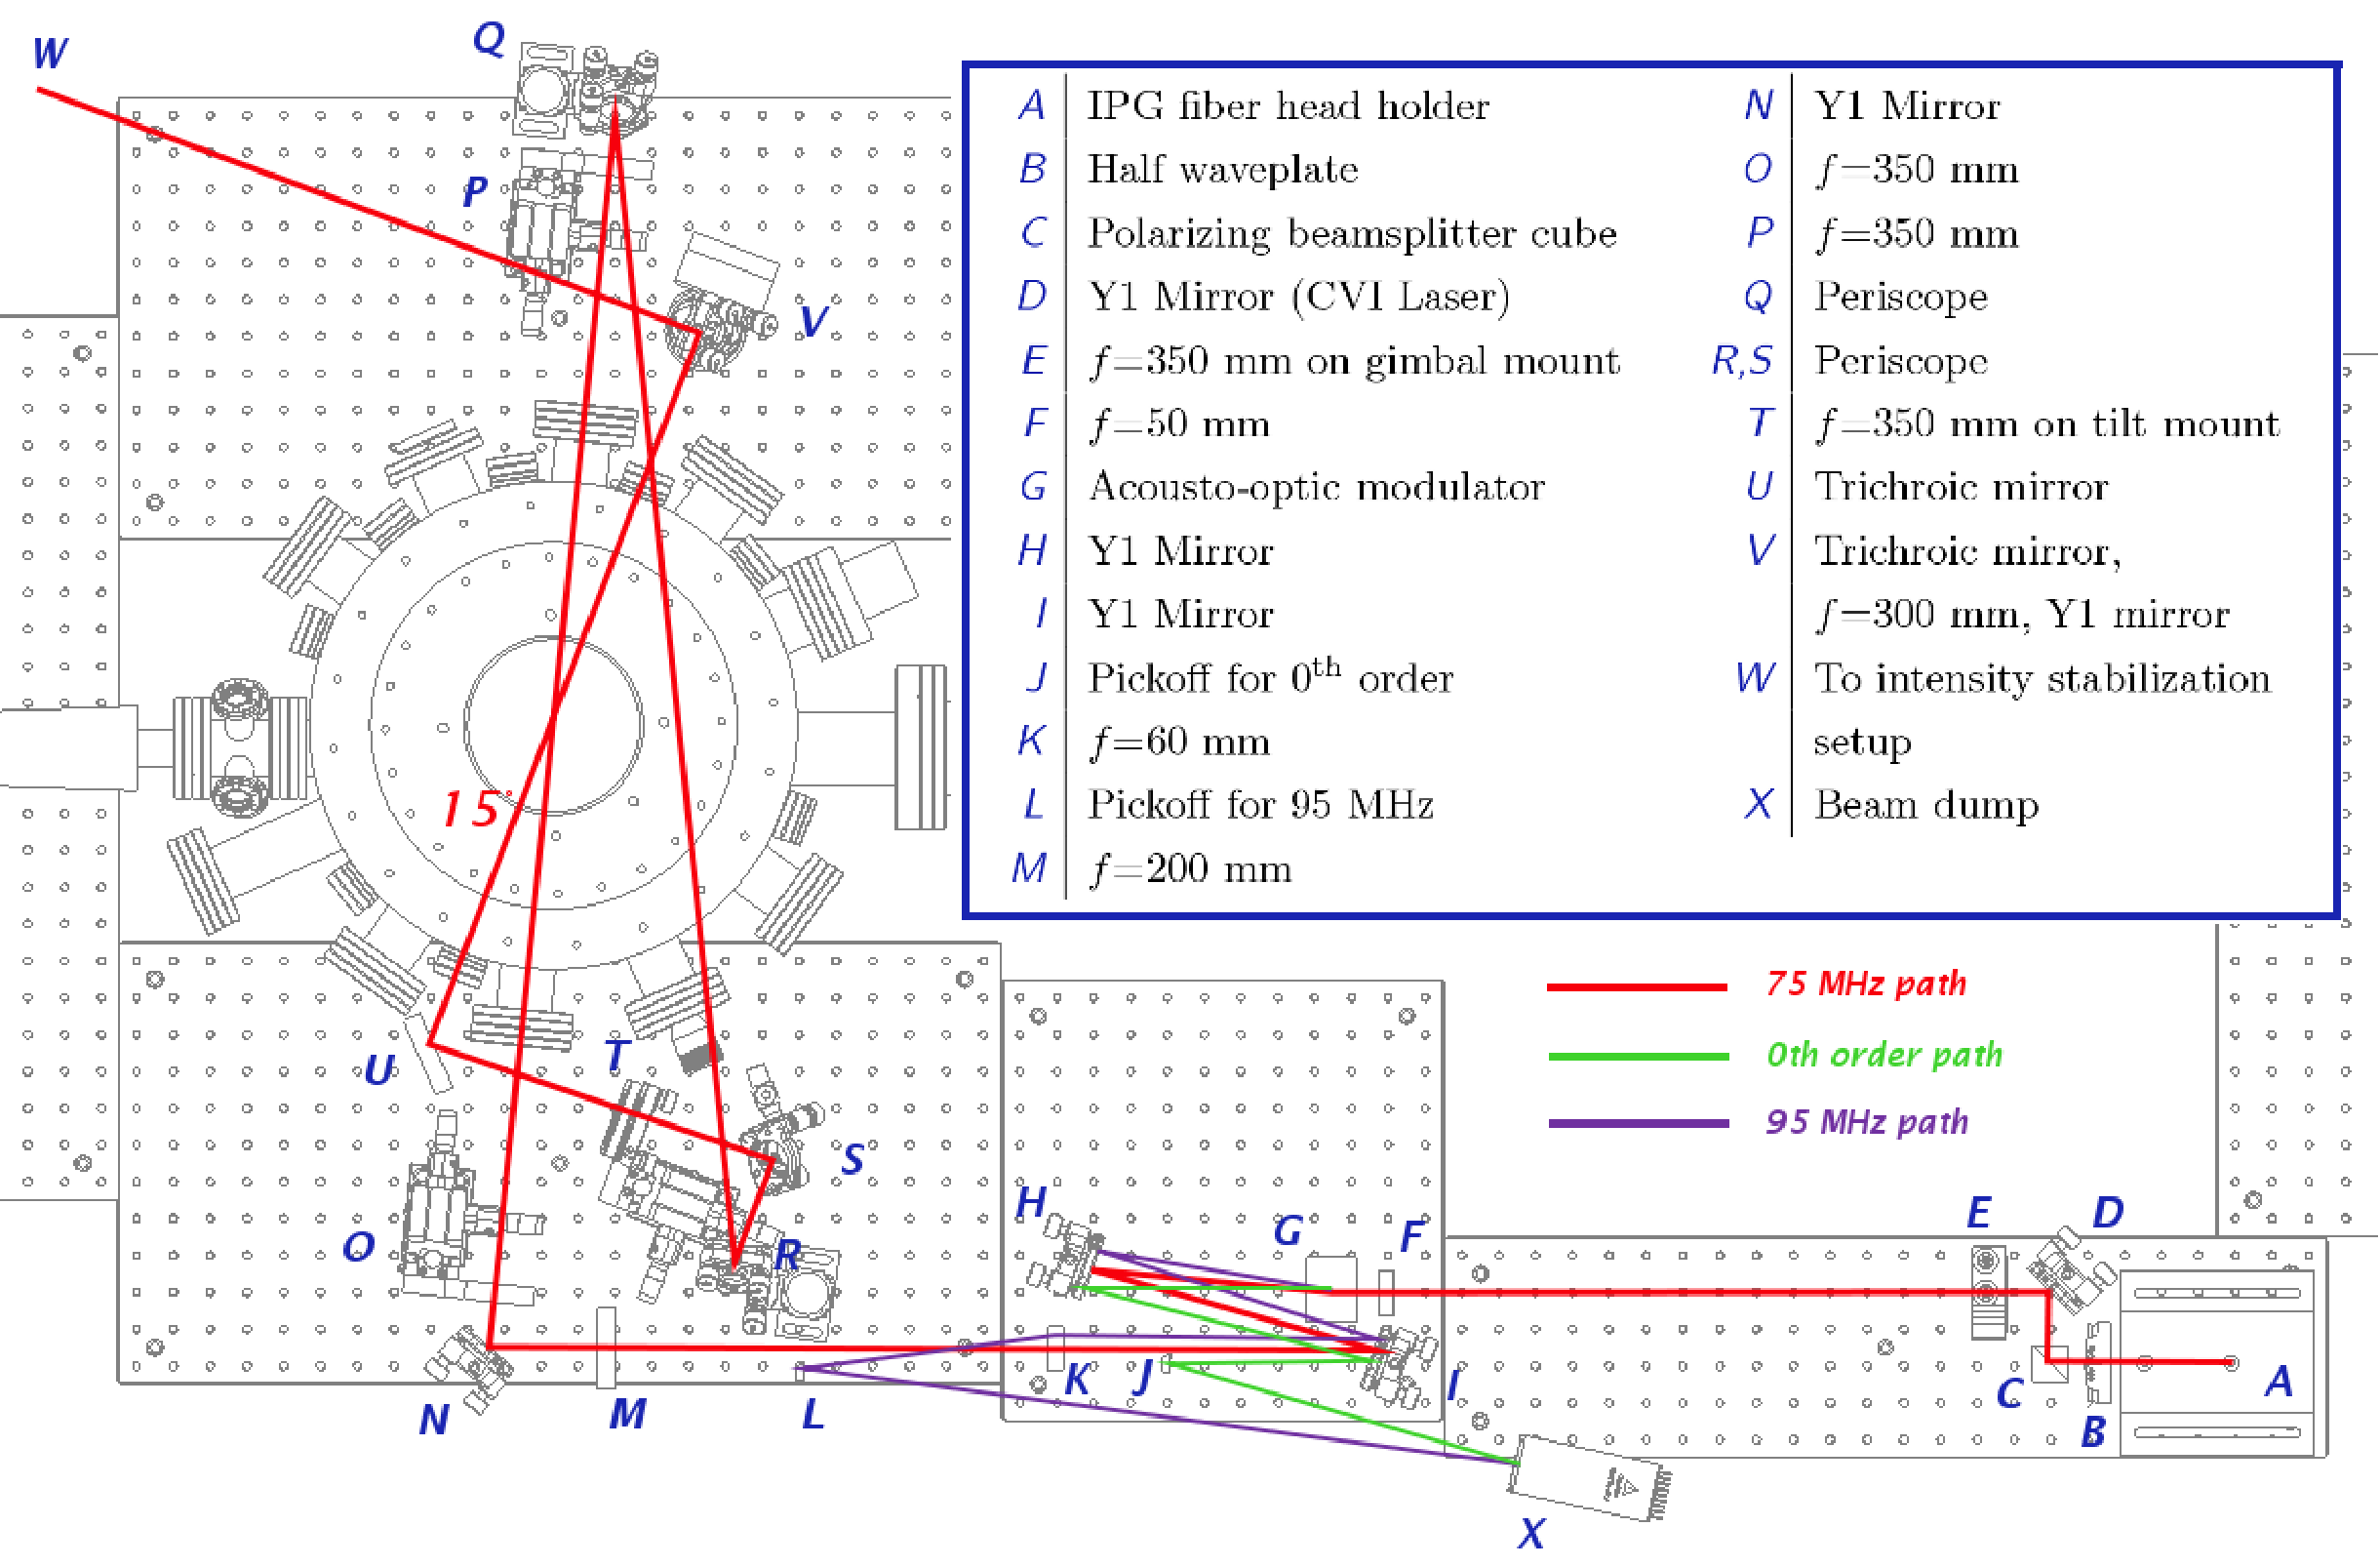
\includegraphics[width=\textwidth]{../masters-figures/odt/opticalsetup/setup.pdf}
\caption[Optical dipole trap setup]{\small Optical dipole trap setup.  The red
lines show the path of the first order of the AOM labeled $G$ when the AOM is
operated at 75~MHz.   Light can be dumped by driving the AOM at 95~MHZ (purple
path) or by turning it off (green path). All mirrors in this setup are Part
Num. Y1-1025-45-UNP from CVI Laser, which have a damage threshold of
10~MW/cm$^{2}$.  All the lens substrates are UV fused silica to reduce power
dissipation and thermal lensing.  The acousto-optic modulator is Part Num.
46080-2-1.06 from Neos Technologies.  } \label{fig:odtsetup}
\end{figure}

\subsubsection{Trap depth and frequencies}

The trapping potential produced by a light field of spatially varying intensity
$I(\bv{r})$ is given by
\begin{equation}
 U_{\mathrm{dip}}(\mathrm{\mathbf{r}} ) =
\frac{\hbar \Gamma^{2}}{4} \left( \frac{1}{\omega_{0}+\omega} +
\frac{1}{\omega_{0}-\omega} \right) \frac{I(\mathrm{\mathbf{r}} )}{\isat} 
\end{equation}
For \li\!\!, a single Gaussian beam of power $P$ and
beam waist $w$, produces a trap depth 
\begin{equation} 
  \frac{U_{0}}{\kb}=\frac{P}{w^{2}} \times
  38.7\times10^{3}  \mu\mathrm{K}\, \mu \mathrm{m}^{2}\, \mathrm{W}^{-1} 
\end{equation}


The first pass through the atoms has 39~W of power and, after losses at
subsequent optics and windows, there are 35~W for the second pass.  The pass
with lower power sets the trap depth,  which is $U_{0}/\kb\approx 280\,\mu$K.  Atoms with an energy higher than $U_{0}$ can escape the intersection
region of the two beams by drifting away along the 39~W beam. 

The trap frequencies are calculated to be approximately 490~Hz and 3750~Hz
along the axial and radial directions of the trap, respectively.  We measured
the radial trap frequency, $\omega_{\mathrm{r}}$, by turning the dipole trap
off briefly (40 $\mu$s) and then turning it back on. The resulting breathing
mode oscillates at twice the radial trap frequency and we obtain
$\omega_{\mathrm{r}} = (2\pi)3.8$~kHz.   The axial trap frequency,
$\omega_{\mathrm{a}}$,  was measured via parametric heating by sinusoidally
modulating the trap depth, and determined to be $\omega_{\mathrm{a}} =
(2\pi)470$~Hz.  



%########################################
\section{Magnetic field}
%########################################

The magnetic field in our experiment is created by a set of coils in
Helmholtz configuration, which sit close to the atoms, inside the recessed top
and bottom viewports of our vacuum chamber (see Fig.~\ref{fig:coilforms}).
\begin{figure} 
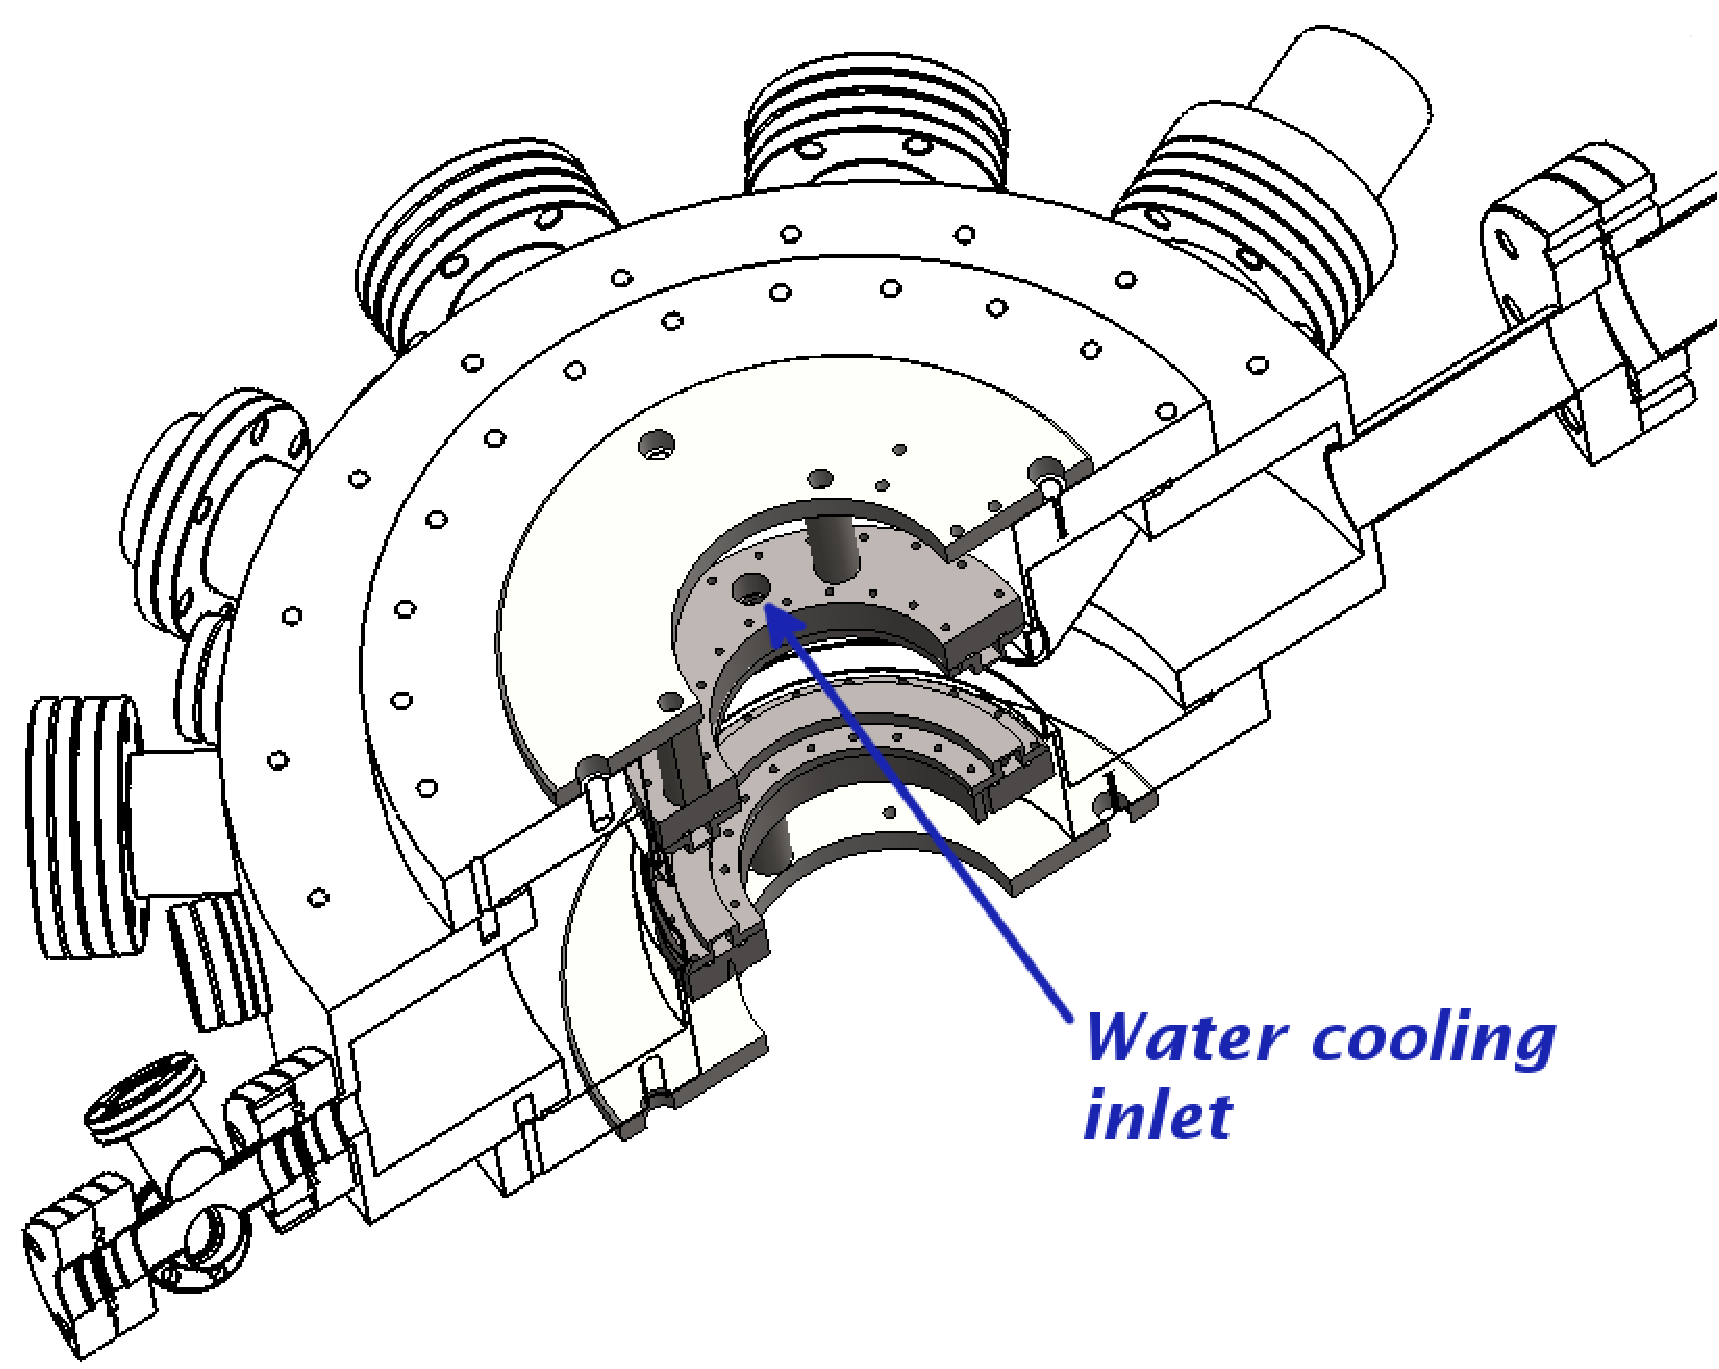
\includegraphics[width=0.45\textwidth]{../masters-figures/coils/angleview.pdf}
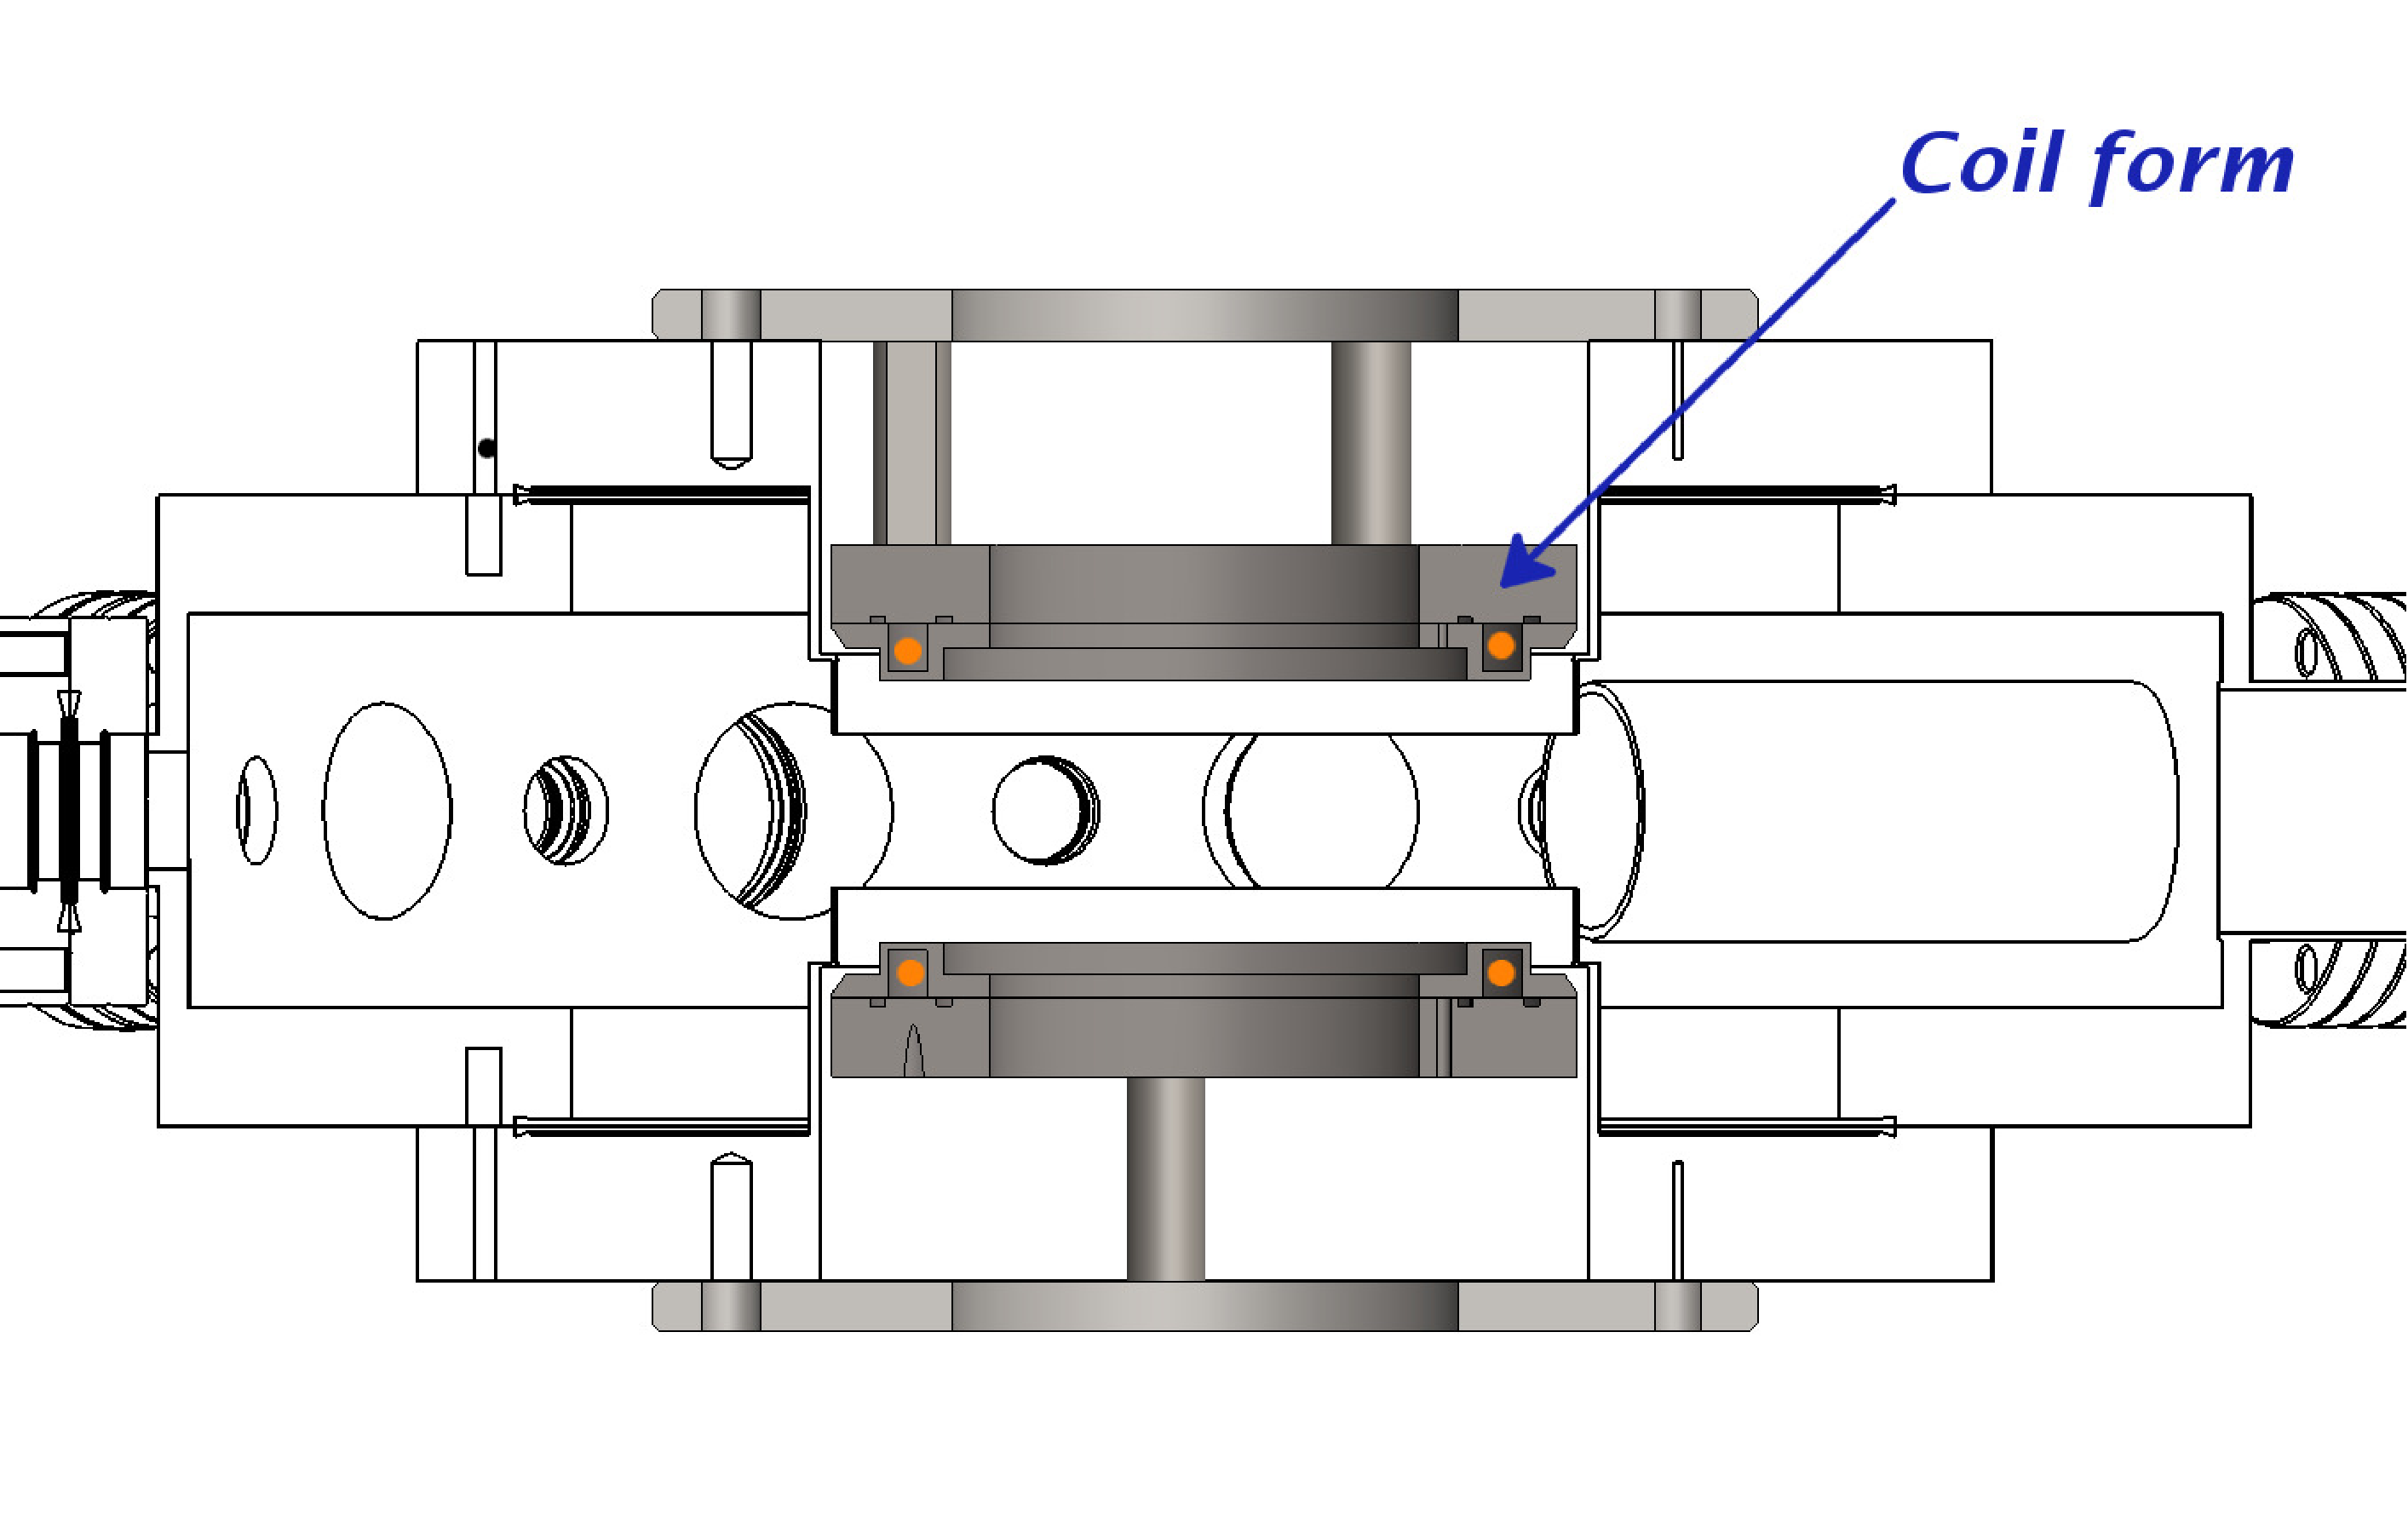
\includegraphics[width=0.55\textwidth]{../masters-figures/coils/sideview.pdf}
\caption[Location of magnetic field coil forms ]{\small Cut-out view of vacuum
chamber showing the location of the coils that create the magnetic field.   The
coil forms are close to the atoms inside the re-entrant top and bottom
viewports.  The forms themselves are attached to a mounting plate that bolts to
the re-entrant viewport flange.  The coils are water cooled.  Only  the water
inlet is shown in this picture, the water outlet is on the half that is cut
out. }
\label{fig:coilforms} 
\end{figure} 
The radius of the coils is 4.72~cm, and is equal to the separation between
them.  There are $n=35$ turns on the top coil and $n-1=34$ turns on the bottom
coil.  As we will see, we take advantage of the mismatch in the number of turns
to levitate the atoms in the latter stages of the experiment.  During the MOT
stages of our experiment, the current through the coils is run such that they
are in anti-Helmholtz configuration. For a current $I$,  the coils produce a
quadrupole magnetic field with a gradient along $z$, given by 
\begin{equation}
 \frac{ \mathrm{d}B_{z}}{ \mathrm{d}z}= \left(
\frac{4}{5} \right) ^{5/2} \frac{3}{4} \frac{\mu_{0} (2n-1) I } { r^{2} } 
\end{equation}
which for $n=35$ and $r=4.72$~cm amounts to 1.72 G/cm/A.

After the optical dipole trap is loaded from the UVMOT the direction of the
current in the top coil is reversed and they produce a bias field given by 
\begin{equation}
 B = \left( \frac{4}{5} \right) ^{3/2} \frac{\mu_{0} (2n-1) I }{2r}  
\end{equation}
 which amounts to  6.8 G/A.   Due to the mismatch in the number of turns
between the two coils, in bias configuration there is a residual gradient given
by 
\begin{equation}
 \frac{ \mathrm{d}B_{z}}{ \mathrm{d}z}= \left(
\frac{4}{5} \right) ^{5/2} \frac{3}{4} \frac{\mu_{0} I } { r^{2} } 
\end{equation}
Fora a bias field of $500-650$~G, where we perform most of our experiments,
this field gradient produces a force on the atoms which is directed upwards and
has about twice the magnitude of the gravitational force.   We have set up
circuitry to controllably shunt some current from the top coil, such that the
atoms are levitated.  
%This is critical for some of our measurements in the
%compensated lattice potential (described in
%Chapter~\ref{chap:compensated-optical-lattice}), where the trapping frequencies
%can be very low.  

The diagram in Fig.~\ref{fig:fieldcircuit} shows a schematic of the magnetic
field system.  The polarity of the current on the top coil is switched by using
an H-bridge made with four field-effect transistors (FETs), labeled $1$ to $4$ in
Fig.~\ref{fig:fieldcircuit}.   FETs labeled 5 and 6 control the amount of
current shunted from the top coil to levitate the atoms.  FETs labeled 7 and 8
control the total amount of current in the system.  
\begin{figure} 
\centering
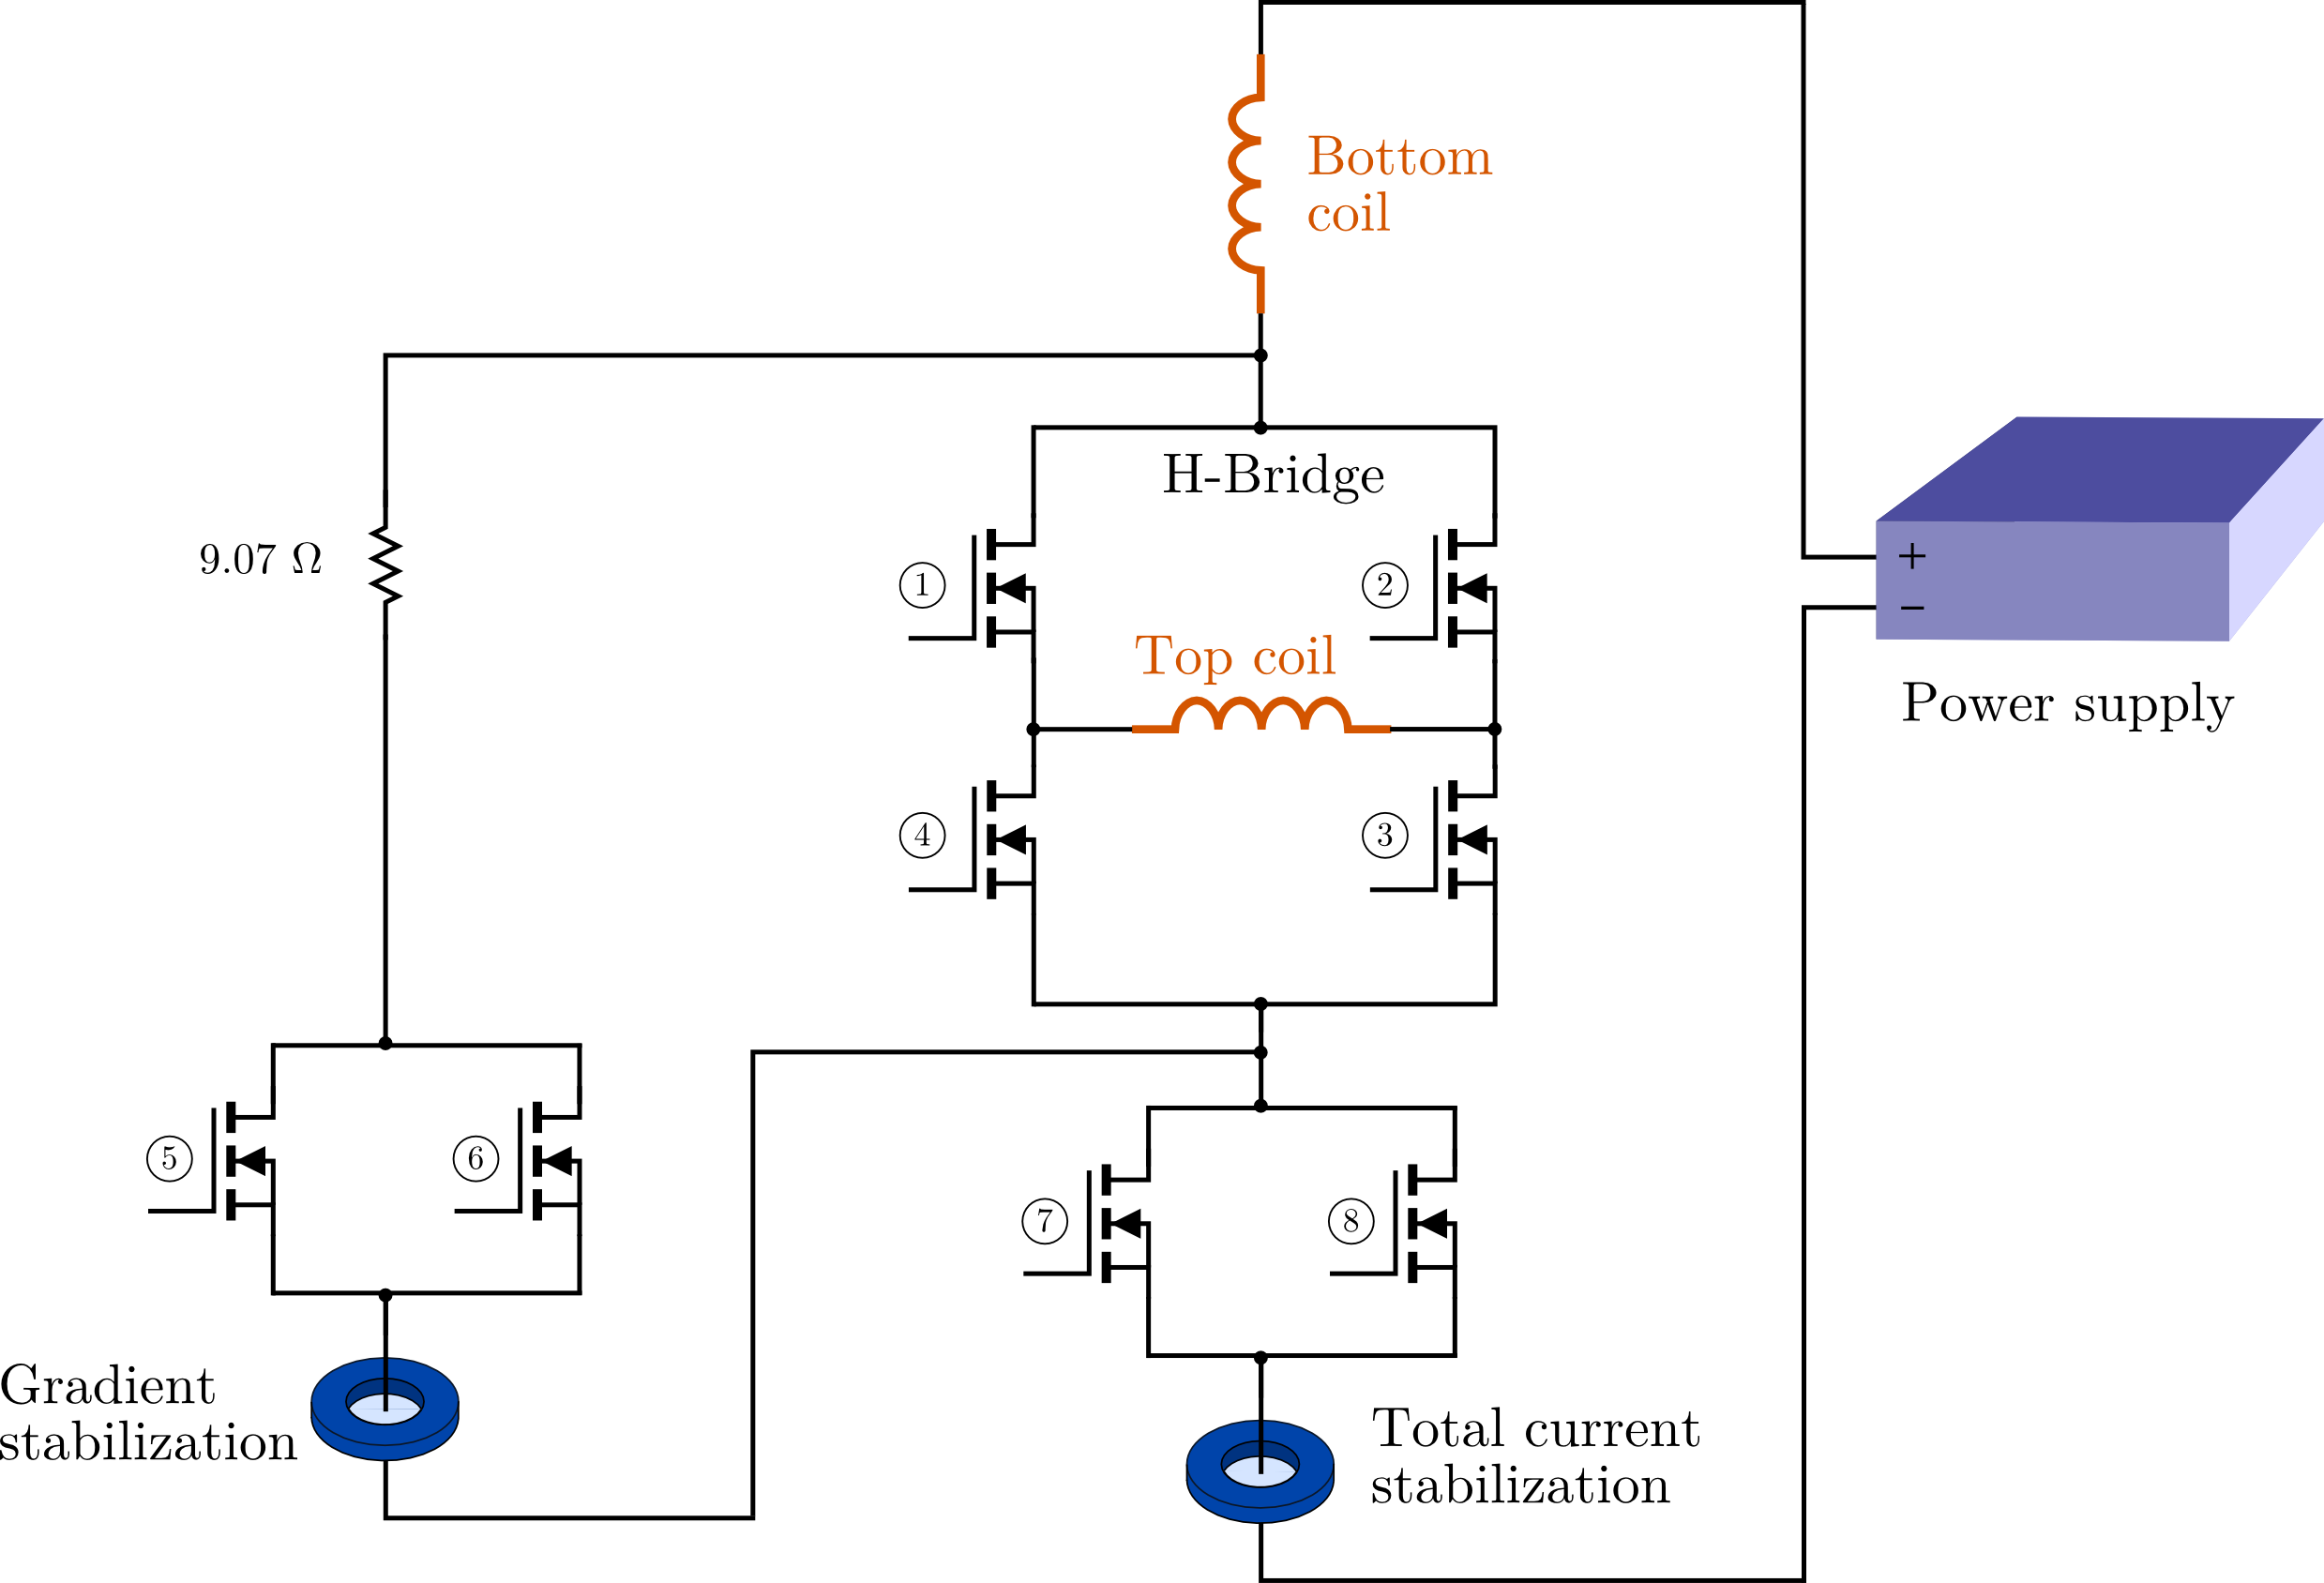
\includegraphics[width=0.85\textwidth]{../masters-figures/coils/fieldcontrol.png}
\caption[Magnetic field control circuit]{\small Schematic of the magnetic field
stabilization circuit.  An H-bridge is used to reverse the polarity of the
current on the top coil.  Current is shunted from the top coil to stabilize the
residual gradient and levitate the atoms.  Current transducers (blue rings) are used
for feedback control of the total current in the system and the current shunted
off the top coil. 
FETs in the H-bridge are Part Num.
STE180NE10.  All other FETs are Part Num. IXFN230N10.  Transient voltage
suppressors, Part Num. 15KW90CA, are used across all the FETs to reduce any
voltage spikes and increase the turn-off speed of the coils.}
\label{fig:fieldcircuit} 
\end{figure} 
The total current through the system is measured  using a Danfisik Ultrastab
866 current transducer, which acts as the source of feedback for stabilization.
For the current shunted for levitation, the transducer used is an LEM HTB-200.
The power supply is a  15~kW Lambda Genesys (80~V, 187.5~A),  operated in
constant voltage mode. A feed forward scheme is implemented to set the voltage
output of the power supply so that the control FETs  do not have to dissipate
too much power.  

%To perform fast magnetic field ramping we override the feed
%forward circuit and set the power supply to a large enough voltage well in
%advance ($\sim$100 ms) for its capacitors to charge up and let the FET's do
%the fast ramping.   In this way we are able to go to from 0 to 120 A in 5 ms.
%although, performing an imaging resonance we find that it takes another 40 ms
%for the field to reach full stability at the top.
%For quick turn off we have
%measured it takes 100 $\mu$s to go from a current of 20 A to zero after
%grounding the gate of the control FETs.  The maximum current we can achieve is
%130 A which can take the field up to 884 G, past the center of the Feshbach
%resonance at 834 G.   



%########################################
\section{Loading the ODT}
\label{sec:odtload}
%########################################

To load the atoms into the ODT one simply needs to turn the ODT light at
maximum power a few ms before the UVMOT is switched on ($t=0$ in the timing
diagram of Fig.~\ref{fig:timingUV}).  We currently turn on the ODT 70~ms before
$t=0$, so it overlaps in time with the 671~nm MOT.  The operation of the 671~nm
MOT is not harmed at all by the presence of the ODT, owing to a small
differential polarizability between the ground $\twos{1/2}$  and excited
$\twop{3/2}$ states~\cite{Safronova2012}.  In other words, both ground and
excited states shift by an equal amount when in the presence of the 1070~nm ODT
light, and thus the laser cooling process is not affected by the presence of
the ODT.   

A wavelength of light where the differential polarizability for a certain
transition vanishes is referred to as a magic wavelength.
Figure~\ref{fig:safronova2p} shows the polarizabilities for the $2S$ and $2P$
states of \li\,  and gives exact values for the magic wavelengths of
$\twop{3/2}$ states.  There is small variability with wavelength around the
wavelength of the ODT (1070~nm),  and the differential polarizability is small.
A calculation (Fig.~\ref{fig:lightshift-calc}) reveals that, for the maximum
intensity of the ODT, a maximum shift of $\sim 1.5\Gamma$ is expected, where
$\Gamma$ is the linewidth of the 671~nm transition. 
\begin{figure}
\centering
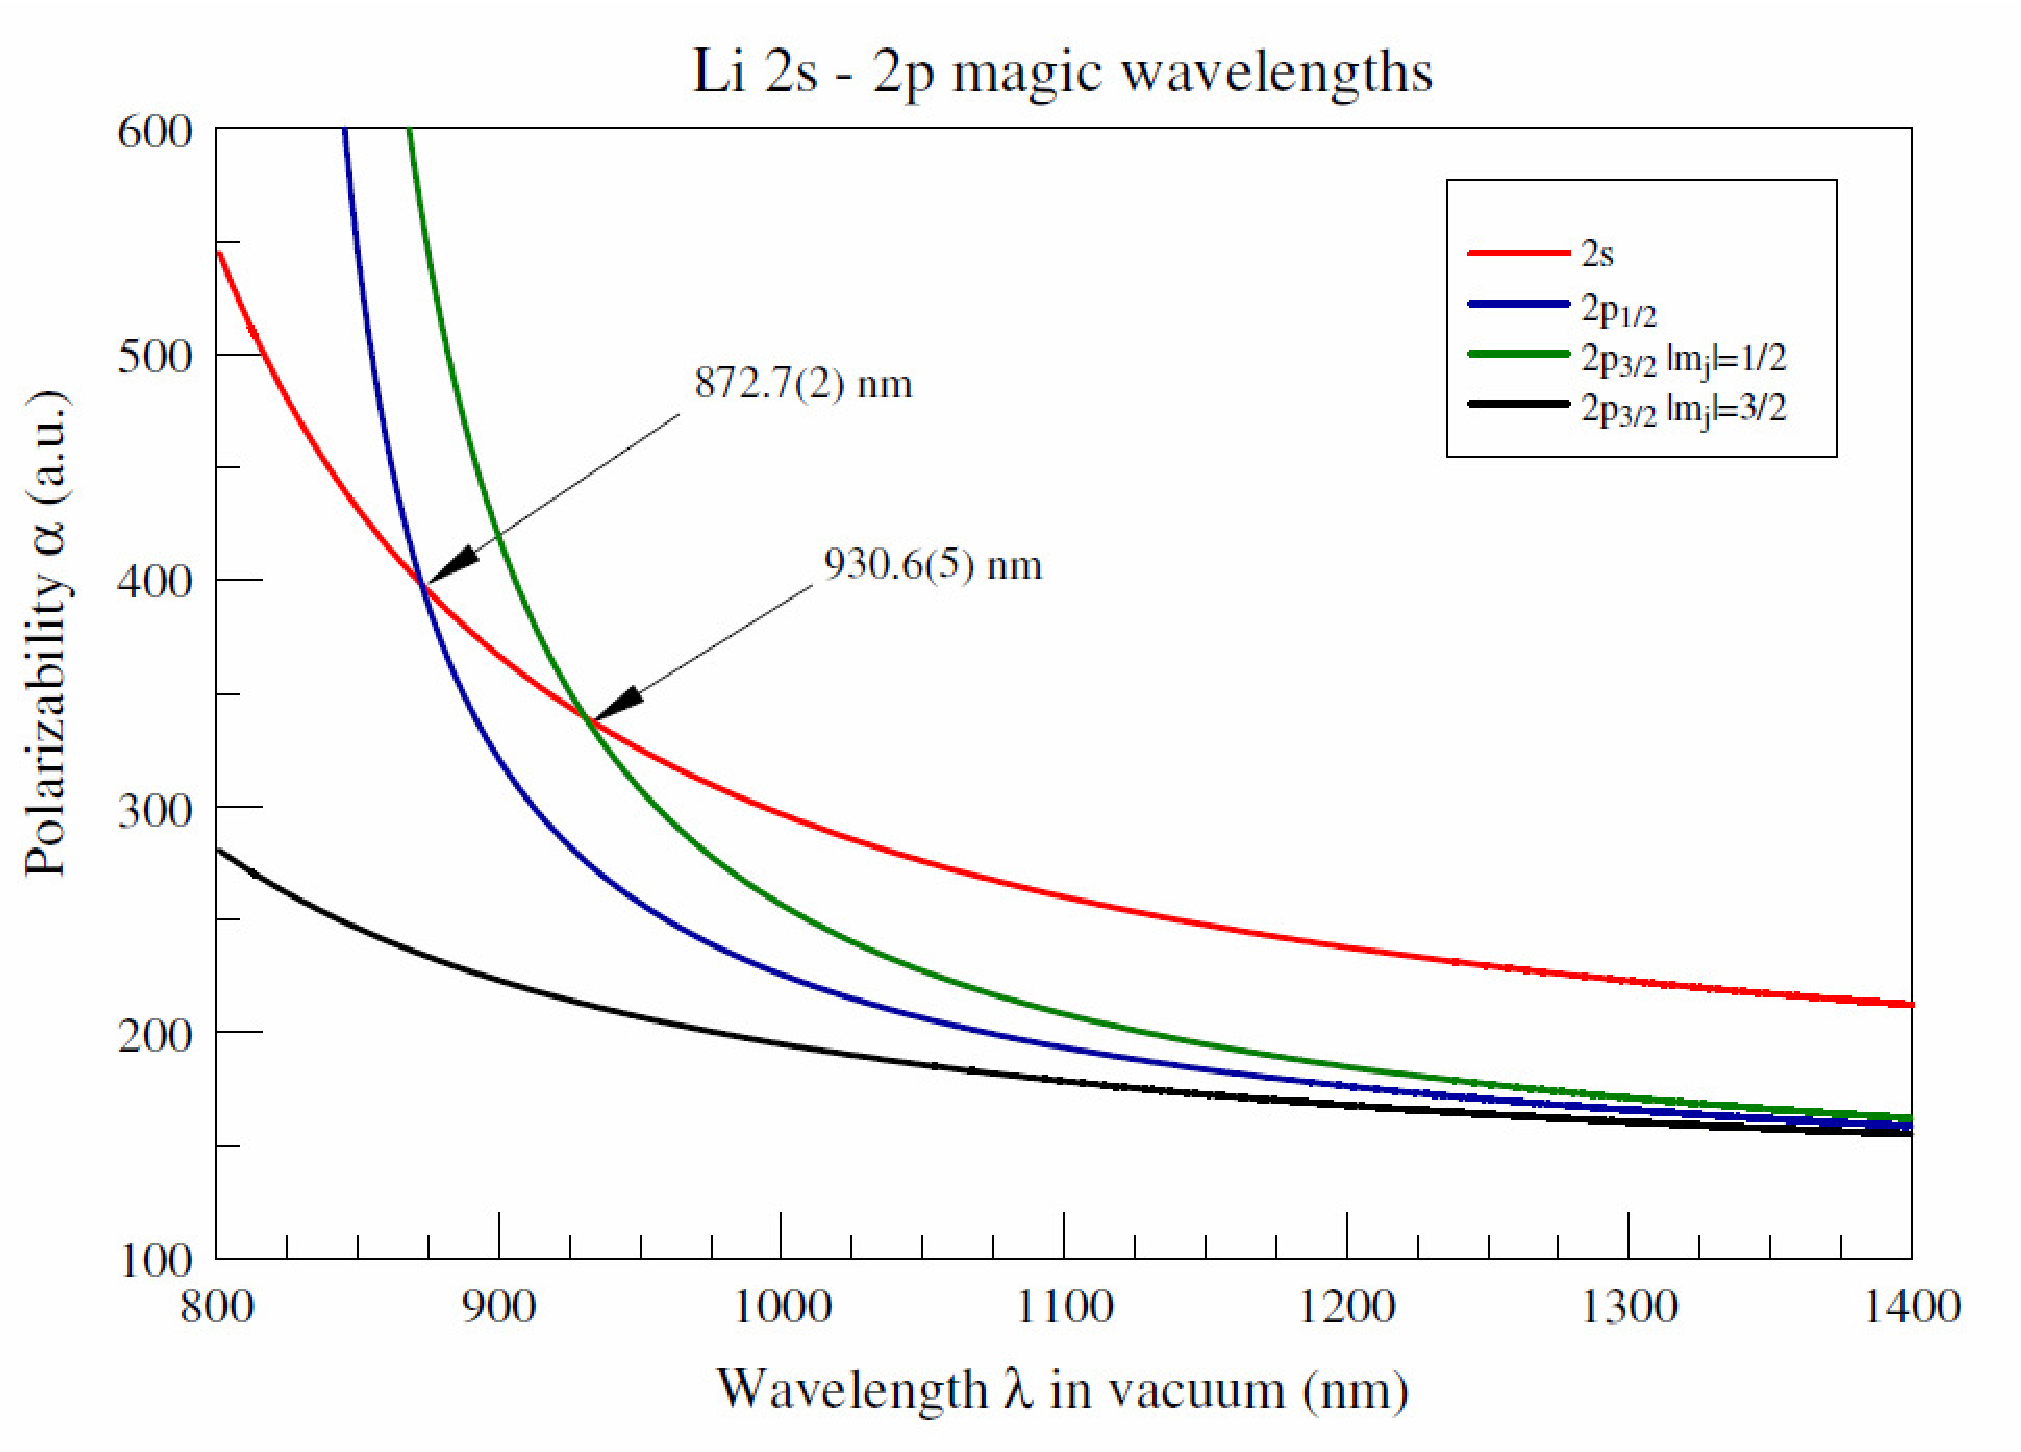
\includegraphics[width=0.65\textwidth]{../masters-figures/safronova/2s2p.pdf}
\caption[Polarizabilities for 1070 nm light]{\small Polarizability in atomic
units for the $2S$ and $2P$ states. Magic wavelengths are indicated by the
arrows.   The atomic units for polarizability (a.u.) can be converted to SI
units (C\,m$^{2}$\,V$^{-1}$) by multiplying by
1.648$\times10^{-41}$~\cite{Safronova2006,Safronova2010}.}
\label{fig:safronova2p} 
\end{figure} 

The situation is different for the \uv\ transition, see
Fig.~\ref{fig:safronova3p}.  In that case, if the wavelength differs much from
a magic wavelength, the differential polarizability of the transition can
become very large.  A calculation for our trap (Fig.~\ref{fig:lightshift-calc})
reveals that for the ODT wavelength of 1070~nm a light shift of at most a few
linewidths is expected at the deepest point in the trap.   It was a great
coincidence that the magic wavelength for the \uv\ transition happened to be so
close to the operating wavelength of our ODT laser.   Being able to continue to
laser cool atoms that are in the volume of the trap greatly enhances the number
of atoms that can be loaded into the ODT,  which can be as large as $\sim
1.4\times 10^{7}$ atoms.  
\begin{figure}
\centering
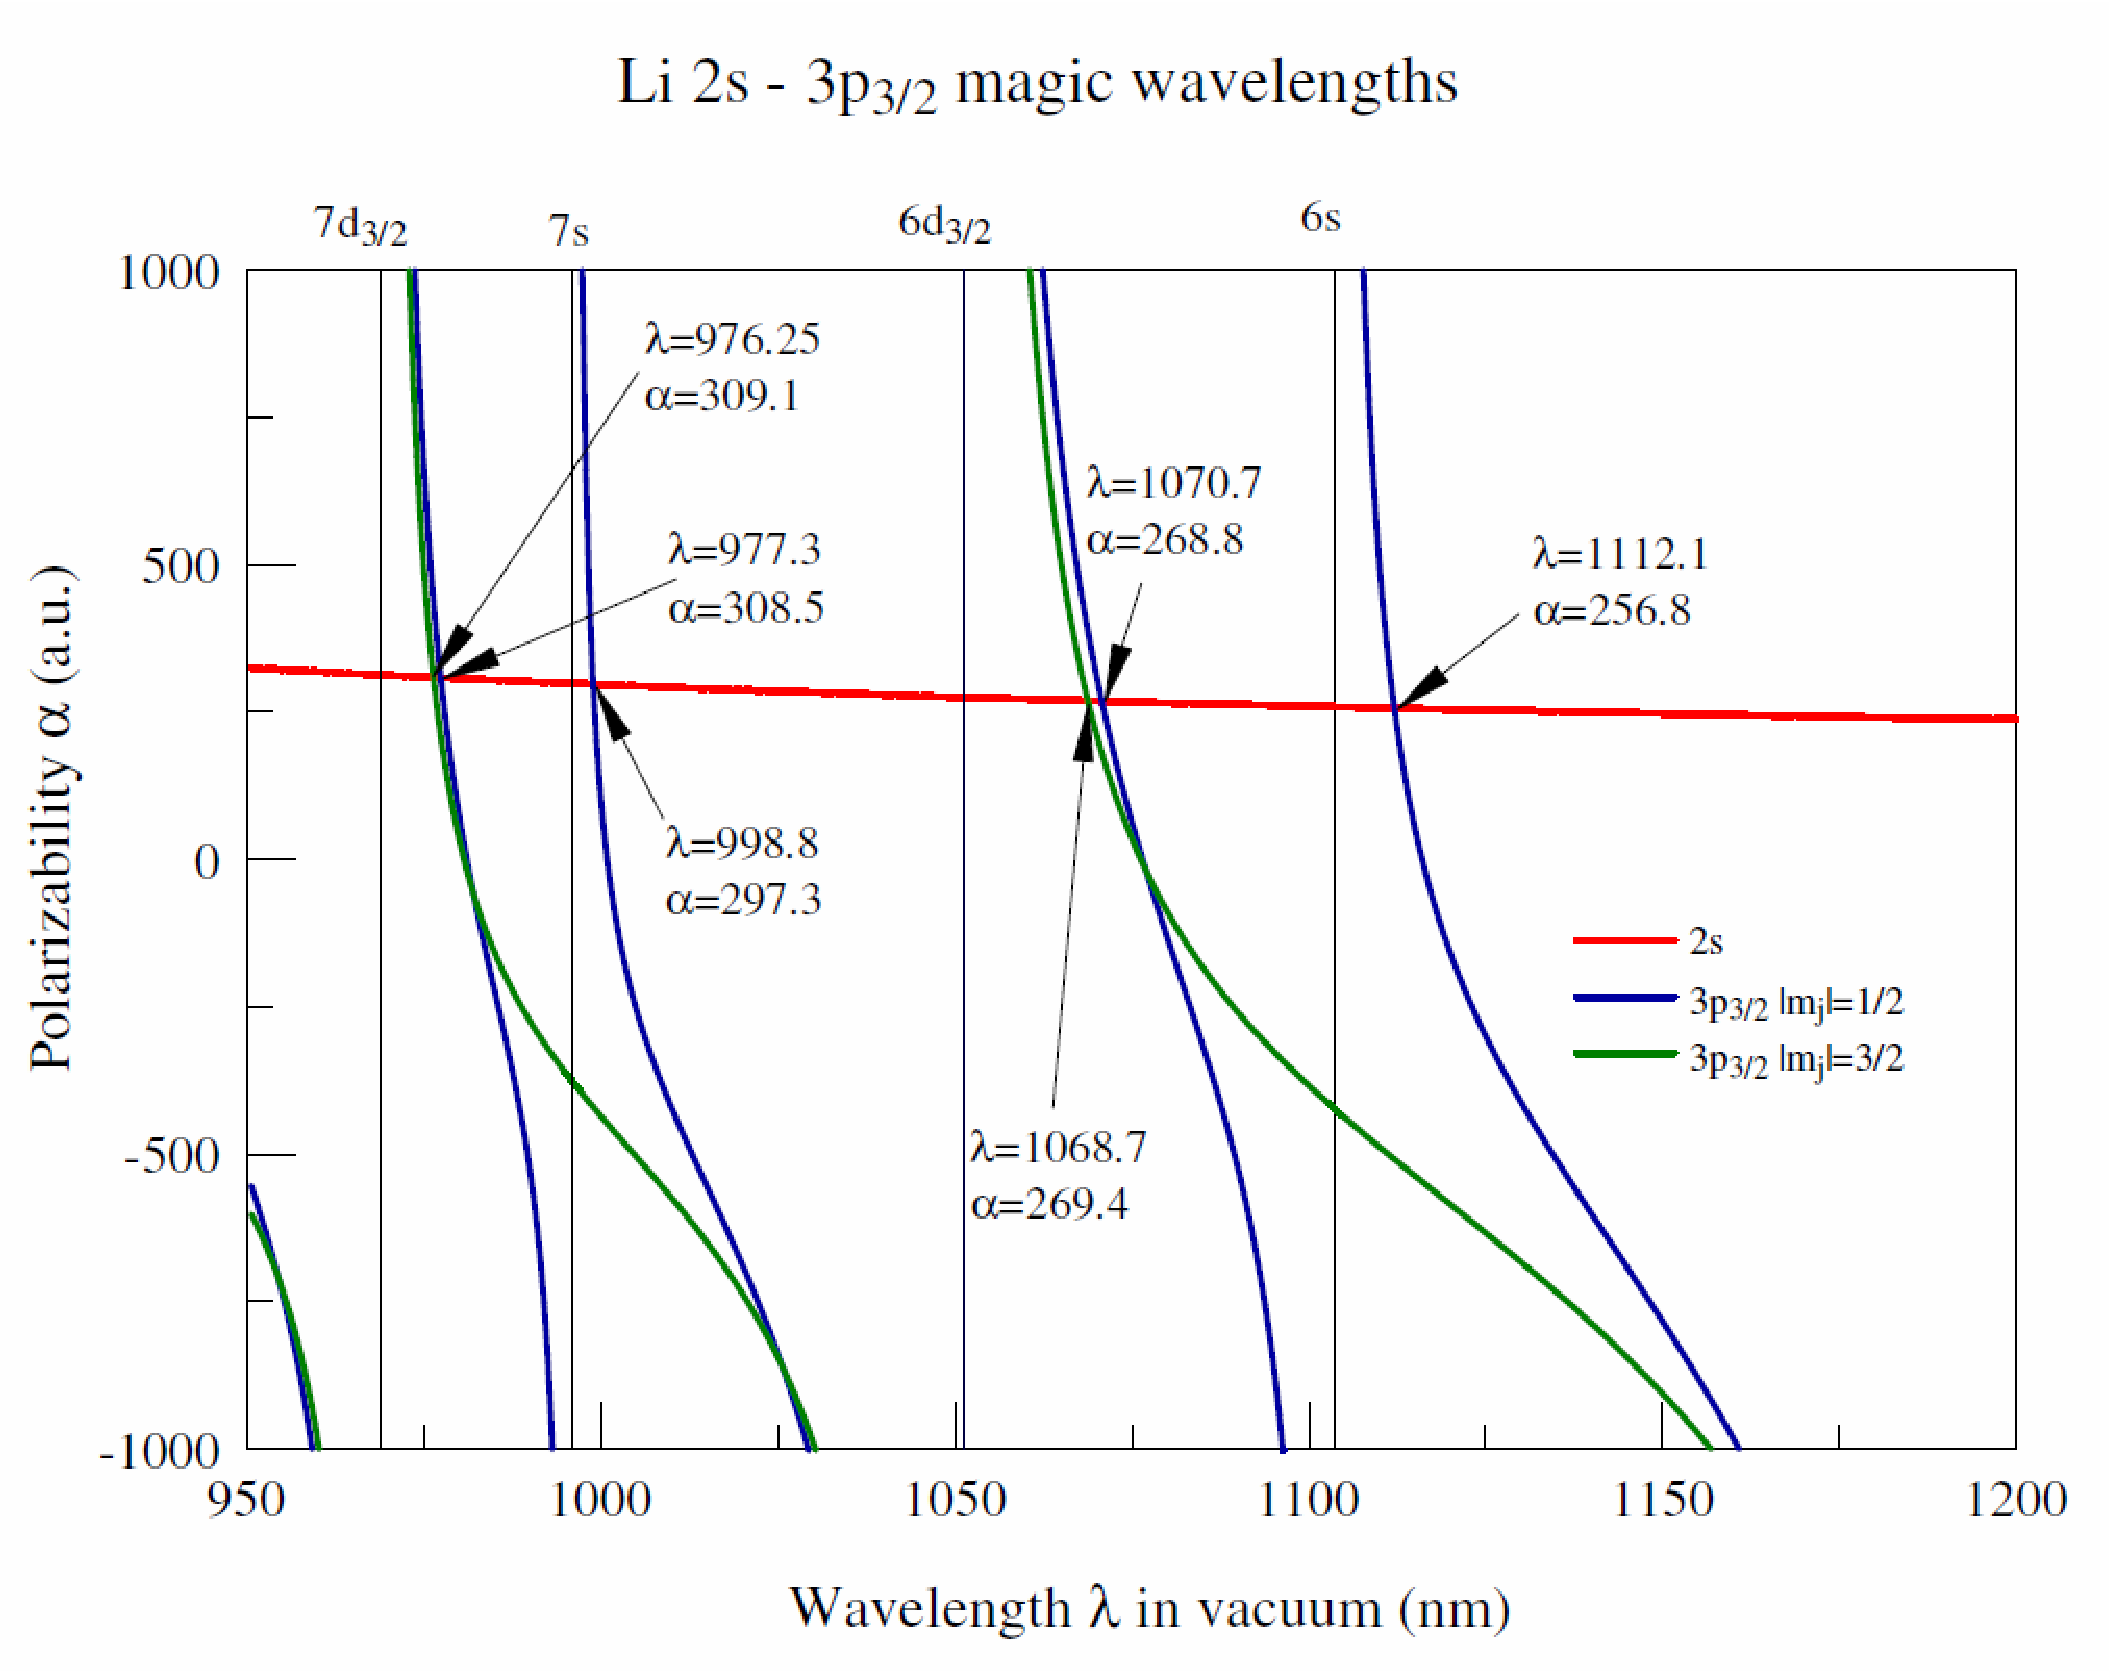
\includegraphics[width=0.65\textwidth]{../masters-figures/safronova/2s3p.pdf}
\caption[Polarizabilities for 1070 nm light]{\small Polarizability in atomic
units of the $2S$ and $3P$ states.  The atomic units for polarizability can be
converted to SI units (C\,m$^{2}$\,V$^{-1}$) by multiplying by
1.648$\times10^{-41}$~\cite{Safronova2006,Safronova2010}.}
\label{fig:safronova3p} 
\end{figure} 

As was briefly mentioned in \S\ref{subsec:mot-uvmot}, we change the detuning of
the 323~nm light in order to optimize the number of atoms loaded into the ODT.
We find that shifting the frequency of the light by $+1$~MHz optimizes
the number loaded.   We also measured the light shift of the \uv\ transition in
our ODT and find that, in the presence of the full power ODT,  the transition
is shifted $\sim 800\,$kHz to the blue,  see Fig.~\ref{fig:lightshift-meas}. 
\begin{figure}
\centering
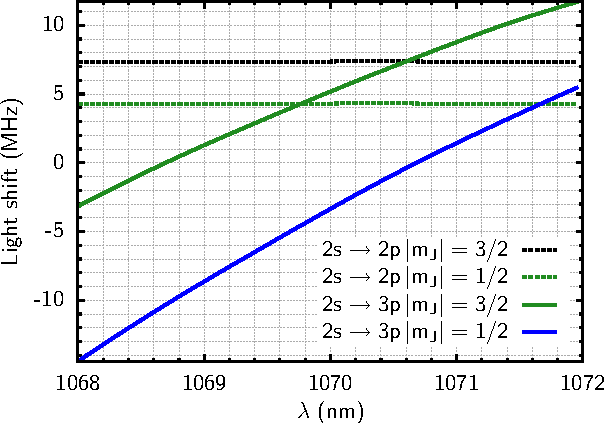
\includegraphics[width=0.6\textwidth]{../masters-figures/safronova/diffpoleps.pdf}
\caption[Differential AC Stark shift for 1070 nm light]{\small Differential AC
Stark shift of the \red and \uv transitions as a function of wavelength for an
intensity of 910 kW/cm$^{2}$ (the maximum intensity the ODT can provide),
calculation by M.~Safronova (personal communication).   }
\label{fig:lightshift-calc} 
\end{figure}
\begin{figure}
\centering
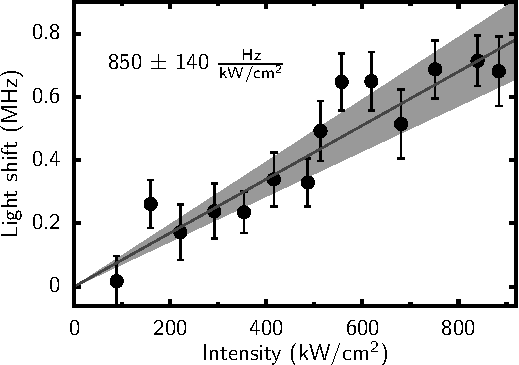
\includegraphics[width=0.6\textwidth]{../masters-figures/lightshift/lightshifteps.pdf}
\caption[Differential AC Stark shift for 1070 nm light]{\small Differential AC
Stark shift of the \uv transition as a function of intensity of the optical
trapping light at $\lambda=1070\,\mathrm{nm}$.  The circles represent the
center of a Gaussian fit of a loss resonance, obtained by heating up atoms in
the ODT with a single UV beam.  The error bars are 1 $\sigma$ statistical error
of the resonance fits.  The solid line is a linear fit to the resonance
position with a slope of $850\pm140 \,\mathrm{Hz/(kW/cm^{2})}$, where the error
(indicated in the plot by the gray shaded area) represents the statistical
uncertainty of the fit and a systematic uncertainty of 10\% on the value of the
trap intensity.  }
\label{fig:lightshift-meas} 
\end{figure}

\subsubsection{Spin mixture} 

Our experiments are realized with a spin mixture of atoms in the two lowest
hyperfine states,  labeled $|1\rangle$ and $|2\rangle$ in
Fig.~\ref{fig:zeemanlevels}.   To create such a spin mixture, we simply turn
off the UV repumping beam 0.5~ms before turning off the UV trapping beam, after
the atoms have been loaded into the ODT.   In that brief time the trapping light
optically pumps all of the atoms into the $F=1/2$ hyperfine state, creating a
balanced mixture of the two hyperfine spin levels. 

After shutting off the UV repumping beam, we turn off the UVMOT magnetic field
gradient, switch the polarity of the top coil,  and ramp up a bias field of
$340~$G, where the scattering length is $\sim -280a_{0}$. The scattering
length is large enough that it leads to efficient evaporative cooling in the
trap.   From this point on, we perform forced evaporation by reducing the power
of the ODT beams.  As the ODT is evaporated away we ramp up a dimple potential,
described in the next section,  such that when the ODT is fully evaporated
away we are left with a degenerate spin mixture in the dimple at a temperature
$T/T_{F}\approx 0.04 $.  The details of the evaporation trajectory will be
discussed later in Chapter~\ref{chap:expprocedures}. 


%########################################
\section{Compensated optical lattice}
%########################################

The compensated optical lattice is the potential in which we realize the
Hubbard model and  carry out all our experiments.   In
Chapter~\ref{chap:compensated-optical-lattice} and Appendix~\ref{app:lattice}
we give much more details about the compensated optical lattice.  In this
section we will give an overview of the setup used to create the potential.

%The optical lattice uses 1064~nm light, red detuned from the 671~nm transition
%such that the light field attracts atoms.   The compensation uses 532~nm light,
%blue detuned from the 671~nm transition, and thus is a potential that repels
%atoms.  

\subsection{Optical lattice and dimple}

An optical lattice potential results due to the stationary interference pattern
of two or more laser beams.   The simplest configuration consists of a laser
beam that is retroreflected upon itself.  We have used this basic
configuration and added a variable liquid crystal retarder LCR, along with a
quarter waveplate and a half waveplate,  in front of the retro-reflection
mirror, as shown in the simplified schematic in Fig.~\ref{fig:simple-latt}.  The
LCR allows us to set the polarization of the retro-reflected beam.  If the
polarization of the retroreflected beam is equal to the polarization of the
incident beam, and both are linear,  then the potential will be a lattice
potential.  On the other hand, if the polarization of the retroreflected beam is
perpendicular to that of the input, there will be no interference and the
potential will be a regular trap.
\begin{figure}
\centering
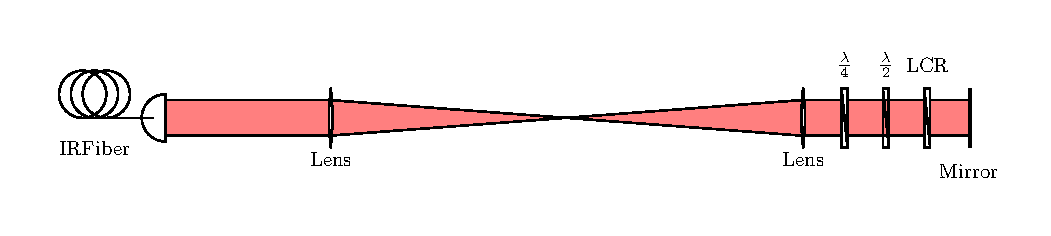
\includegraphics[width=0.8\textwidth]{../ernie-figures/lattice/simple-assembly/latticesassembly.pdf}
\caption[Simplified lattice axis]{\small Simplified setup for a one-dimensional
lattice.   In our implementation we have included waveplates and a variable
liquid crystal retarder (LCR). This allows us to control the polarization of
the retroreflection.  }
\label{fig:simple-latt} 
\end{figure}

We have setups like the one shown in Fig.~\ref{fig:simple-latt} along three
orthogonal axes in order to form a simple cubic lattice potential.   The waist
of each beam is $\sim45\mu$m and thus the intersection region of all three
beams is quite small.  When the polarization of the retro beams is set
perpendicular to the input polarization, we refer to the trap formed at the
intersection of all three axes as the \textbf{dimple trap}.  The dimple trap
provides an excellent starting point for our experiments.   The large
confinement strength resulting from the small volume of the trap leads to efficient
evaporation.  In the dimple we can routinely achieve temperatures as low as
$T/T_{F}\approx 0.04$.  By comparison, in the ODT  one has to spend
considerable effort optimizing the evaporation trajectory, alignment, and beam
profile of the ODT beams to get below $T/T_{F}\approx0.05$, and routinely the
ODT can only get down to $T/T_{F}\approx 0.15$. 


\subsection{Compensation} 

The compensation is a repulsive potential used to tune the amount of
confinement produced by the optical lattice.  An illustration of this idea is
shown in Fig.~\ref{fig:green-push-cartoon}. 
\begin{figure}
\centering
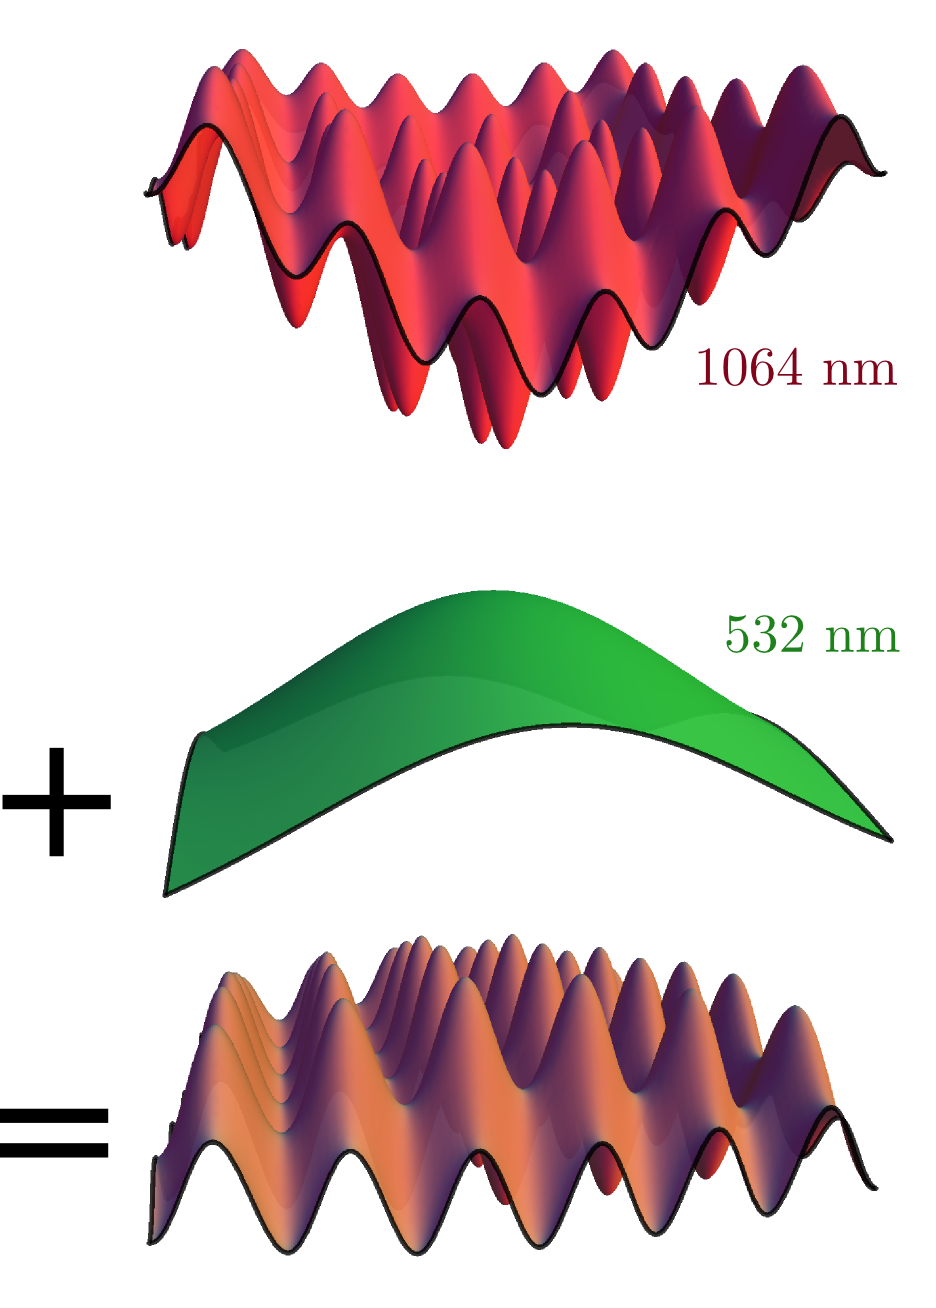
\includegraphics[width=0.35\textwidth]{../figures/setup-overview/compensation-push-cartoon.png}
\caption[Compensation]{\small Illustration of the concept behind a compensated
optical lattice. }  
\label{fig:green-push-cartoon} 
\end{figure}
Adjusting the density of the sample is critical when trying to access the
different phases of the Hubbard model.  Furthermore the compensation was
designed such that it enables the possibility of continuing to evaporatively
cool the atoms once they are in the lattice potential (this will be discussed
in Chapter~\ref{chap:compensated-optical-lattice}.  Reaching lower temperatures
in an optical lattice is a major goal for quantum simulation with ultracold
atoms. 

The compensating potential is formed by Gaussian beams that co-propagate with
the incident lattice beams but are not retroreflected.  A schematic of the
compensation plus optical lattice setup is shown in
Fig.~\ref{fig:comp-latt-schem}.   The details of this setup are described in
detail in Ernie Yang's Master's thesis~\cite{ErnieMs}.  
\begin{figure}
\centering
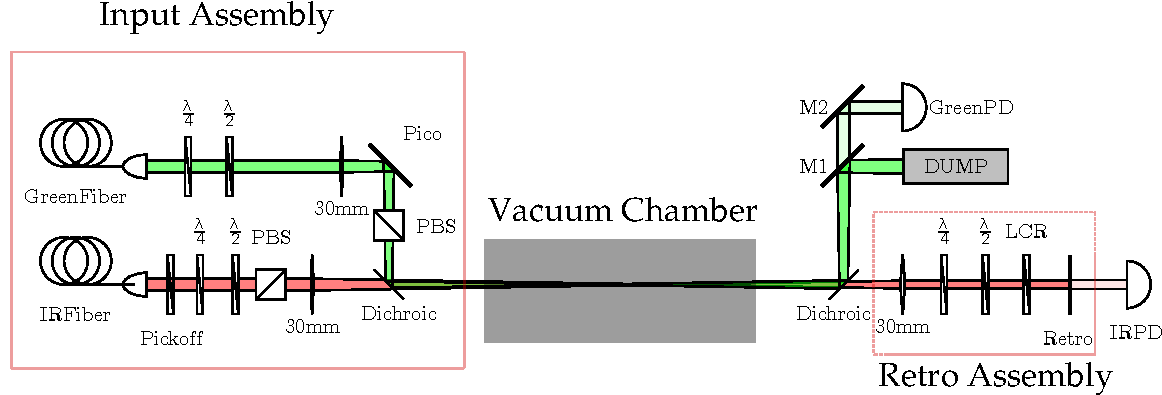
\includegraphics[width=0.8\textwidth]{../ernie-figures/lattice/assembly/latticesassembly.pdf}
\caption[Compensated lattice axis]{\small Compensated optical lattice setup
along one of the three axes.  More details regarding the construction of the
setup can be found in Ernie Yang's Master's thesis~\cite{ErnieMs}}
\label{fig:comp-latt-schem} 
\end{figure}
The light that is coming out of the fibers in Fig.~\ref{fig:comp-latt-schem} is
prepared in a separate optical table.  For the lattice we use 1064~nm light
from a single mode IPG Photonics fiber laser.   The optical layout is shown in
Fig.~\ref{fig:1064setup}.   For the compensation we use 532~nm light from a
Coherent Verdi.  The optical layout is shown in Fig.~\ref{fig:532setup}. 
 
\begin{figure}
\centering
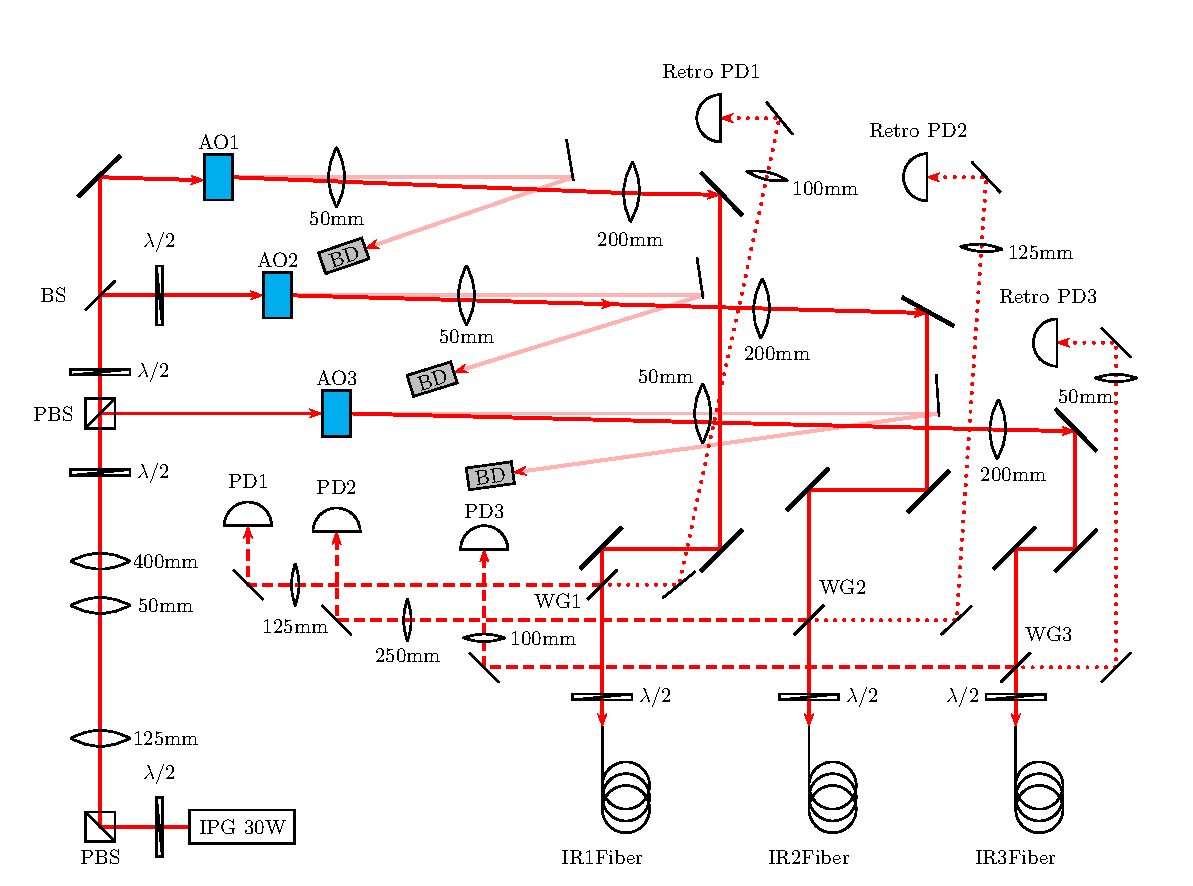
\includegraphics[width=\textwidth]{../ernie-figures/lattice/setup/lattices.pdf}
\caption[1064~nm setup]{\small Optical setup showing how the 1064~nm light from
the 30~W IPG laser is split up before coupling into the fibers for each of the
three lattice axes. The acousto-optic modulators, labeled AO1-3, are used for
intensity stabilization of the intensity.   Feedback to these AOs comes from
the photodetector labeled IRPD in Fig.~\ref{fig:comp-latt-schem}.  The driving
frequencies of AOs 1-3 is 70, 80, and 90 MHz respectively, with the offset used
to avoid interference between the different lattice axes.  }
\label{fig:1064setup} 
\end{figure}
\begin{figure}
\centering
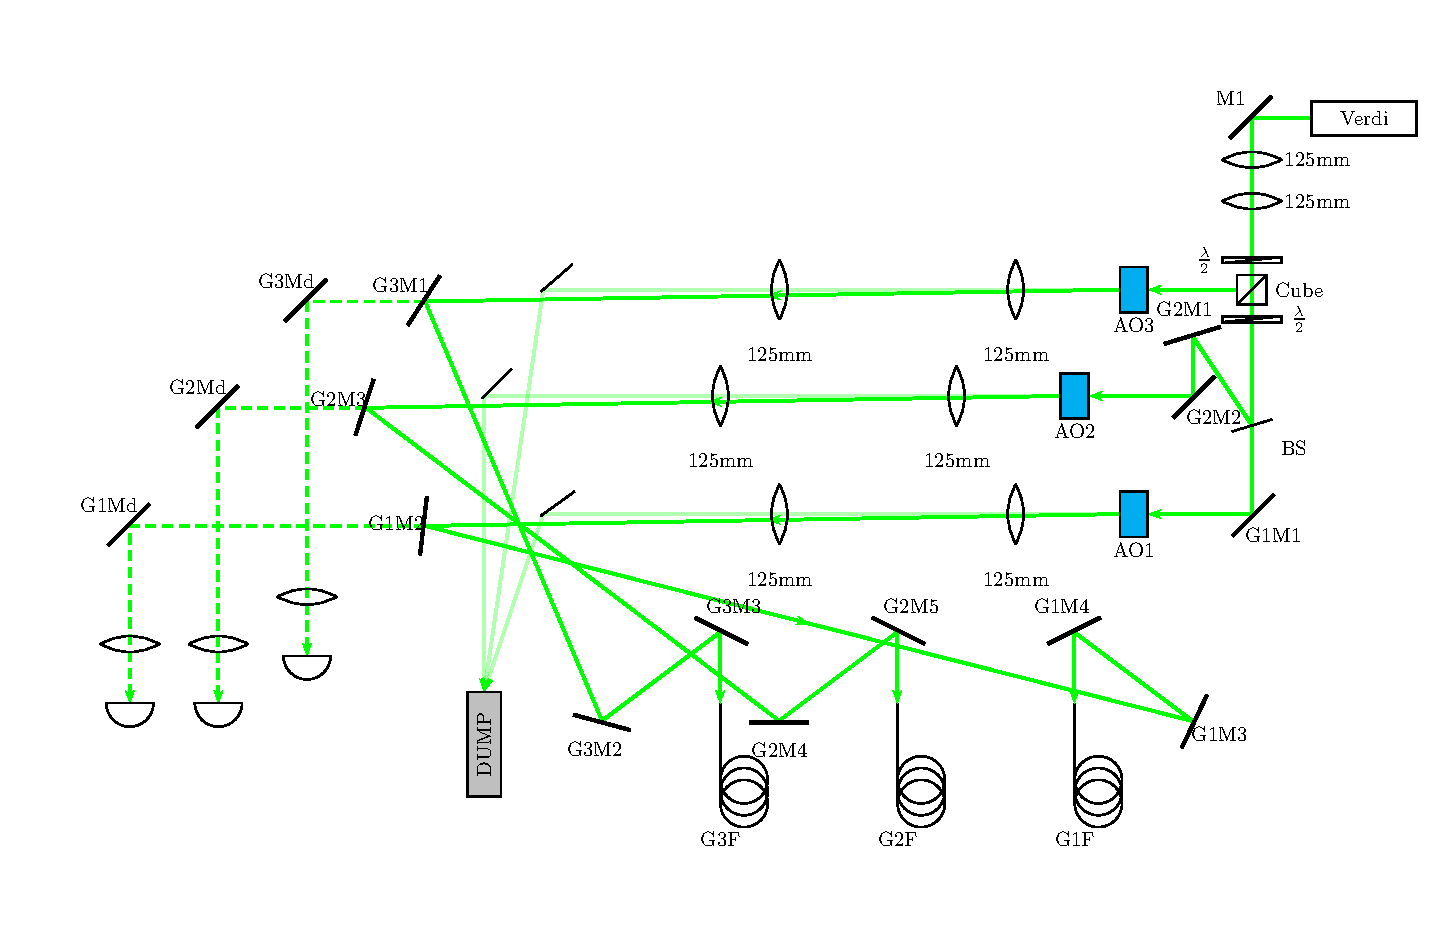
\includegraphics[width=\textwidth]{../ernie-figures/lattice/setup/green.pdf}
\caption[532~nm setup]{\small Optical setup showing how the 532~nm light from
the Coherent Verdi is split up before coupling into the fibers for each of the
three lattice axes. The acousto-optic modulators, labeled AO1-3, are used for
intensity stabilization of the intensity.   Feedback to these AO's comes from
the photodetector labeled GreenPD in Fig.~\ref{fig:comp-latt-schem}. The
driving frequencies of AOs 1-3 is 80, 88, and 72 MHz respectively, with the
offset used to avoid interference between the different compensation axes. }
\label{fig:532setup} 
\end{figure}




%########################################
\section{Diagnostics}
%########################################

Having described all the systems that we use to manipulate the atoms, we will
now describe very generally the systems used to measure their properties.  For
diagnostics we exploit again the strong interaction of the atoms with near
resonant light.   We can perform fluorescence, absorption and phase contrast
imaging of the atoms.   We have also built a setup to measure  Bragg scattering
of light, a probe of the crystalline and spin order of atoms in a
lattice~\cite{Ted2010}. A detailed description of the Bragg scattering setup will be
presented in Chapter~\ref{chap:bragg-scatt}.    

For the purposes of imaging the MOT and UVMOT, which can reach a spatial extent
of up to several mm after TOF expansion, we use fluorescence imaging
using a surveillance CCD camera, see Fig.~\ref{fig:diagnostics}. 

To image the smaller samples (tens of $\mu$m) in the ODT, the dimple, or the
optical lattice,  we use a nearly diffraction limited relay lens system
(Fig.~\ref{fig:relaylens}) which creates a real image of the atoms outside the
vacuum chamber.  The numerical aperture (NA=0.16) of the relay lens determines
the resolution of the imaging system
($\sigma_{\mathrm{res}}\approx3\,\mu$m)\footnote{Here the resolution of the
imaging system is defined as the $1/e$ radius of the point-spread function PSF
of the imaging system, $\mathrm{PSF}(x)\propto \exp\left[
-\frac{x^{2}}{\sigma_{\mathrm{res}}^{2}} \right]$.  The size of the PSF was
obtained by fitting images of a 1951 USAF test target.}.   A commercial
microscope objective is then used, in conjunction with a Nikon telephoto lens,
to image the the relayed image of the atoms onto a CCD.   The setup is shown in
Fig.~\ref{fig:diagnostics}, 

\begin{figure}
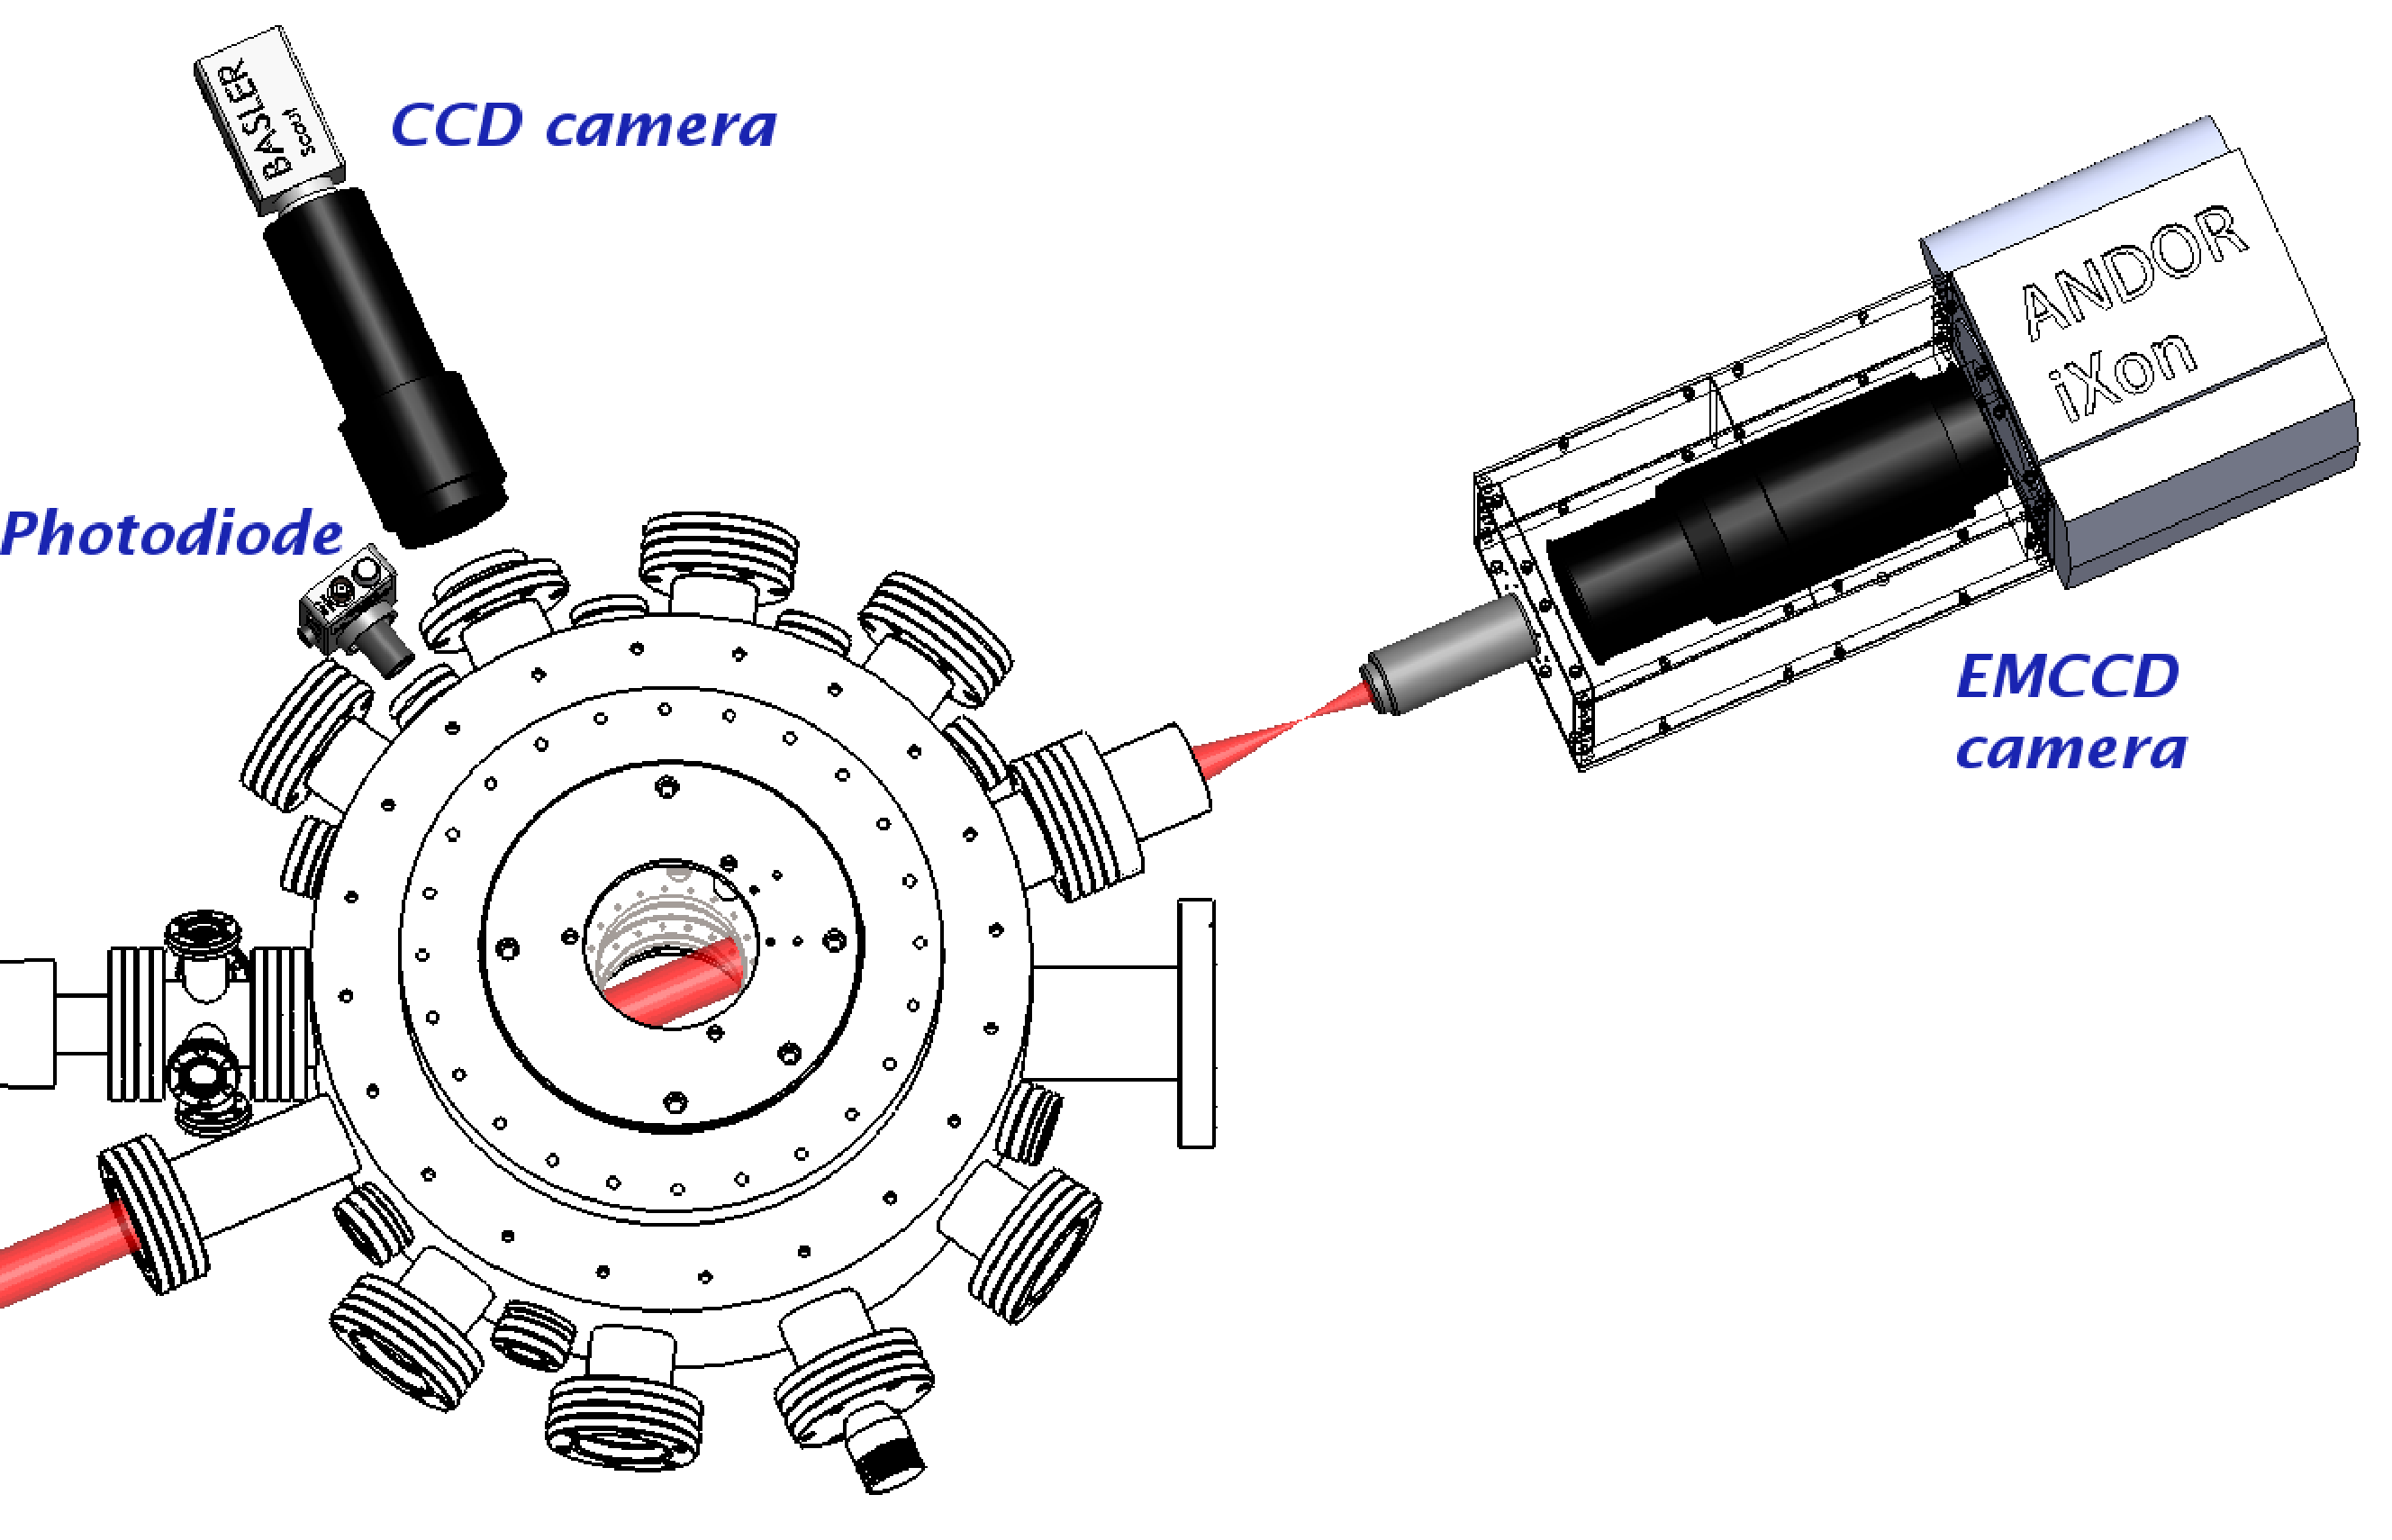
\includegraphics[width=\textwidth]{../masters-figures/imaging/setup.pdf}
\caption[Diagnostics setup]{\small This figure shows instruments that we use
for diagnostics.  A photodiode can be used for basic monitoring of the MOT
loading level.  Fluorescence imaging with the Basler CCD camera is used to
characterize the MOT and UVMOT.   Smaller samples in the ODT and optical
lattice are imaged using a relay lens (not shown). A microscope objective and
Nikon telephoto lens, project the image of the atoms onto the Andor iXon EMCCD
camera (DU-897-E).}  
\label{fig:diagnostics} 
\end{figure}
 
\begin{figure} \centering
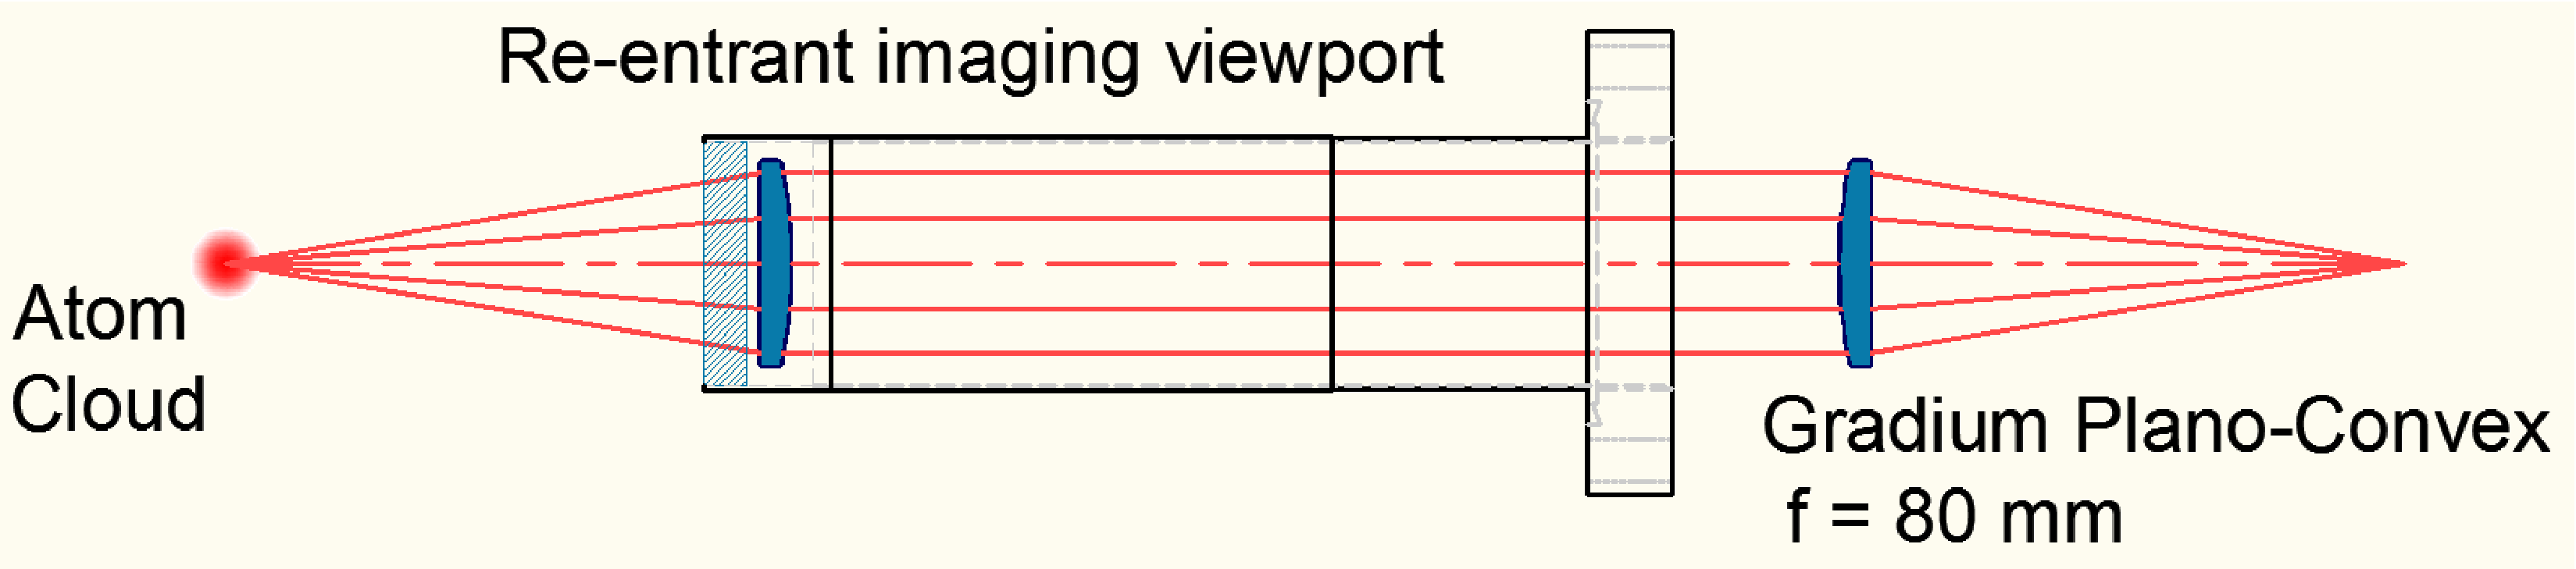
\includegraphics[width=0.85\textwidth]{../masters-figures/imaging/relay.pdf}
\caption[Relay lens system]{\small  Relay lens system to form an image of the
atoms outside the vacuum chamber. A re-entrant imaging viewport on the vacuum
chamber allows placing a 1 inch diameter lens 80~mm away from the atom sample.
Both lenses are Part Num. GPX-30-80 gradient index plano-convex lenses from
LightPath Technologies.  }
\label{fig:relaylens} \end{figure} 



%########################################
\section{Control, automation, and data analysis}
%########################################

Finally, we describe the computer control system that orchestrates the
behavior of all other systems in our experiment.   The control system is is
based on the National Instruments PXI chassis NI-PXIe1062Q.   

The chassis hosts
three 6733 Analog Output cards and a 6259 Multifunction DAQ card.   An experimental
sequence consists of a series of TTL pulses that control the timing of events
related to instruments on the apparatus.  The clock to which TTL pulses are
synchronized is an 80~MHz oscillator on the 6259 Multifunction DAQ card.    A
digital sequence can have a maximum output rate of 10 MHz (resolution time step
of 1 $\mu$s) and at this output rate the buffer can hold sequences that last
several tens of seconds.  We use the analog output channels of the PXI system
as one typically uses arbitrary waveform generators; waveform outputs can be
triggered by TTL pulses at any given time during the experimental sequence.
The timebase for arbitrary waveform outputs on analog output channels is the
on-board oscillator of each card.  For the 6259 it is a 80~MHz oscillator and
for the 6733 it is a 20~MHz oscillator.  

The experimental sequences, including all waveform outputs,  are programmed in
a format based on the Python programming language.  This makes it very easy to
program new sequences and recycle parts of old sequences.    The Python  based
sequence code is interpreted by a program also written in Python which produces
a raw sequence output file that contains all the TTL timings and the waveforms
for a particular experiment.  The raw sequence output is read by LabVIEW, which
takes care of outputting the sequence on the TTL and analog output channels.  

In an experimental cycle, the MOT is loaded until a certain fluorescence is
reached. At that point a trigger synchronized with the 60~Hz mains starts the
output of the experimental sequence. 


